% Options for packages loaded elsewhere
\PassOptionsToPackage{unicode}{hyperref}
\PassOptionsToPackage{hyphens}{url}
\PassOptionsToPackage{dvipsnames,svgnames,x11names}{xcolor}
%
\documentclass[
  letterpaper,
  DIV=11,
  numbers=noendperiod]{scrartcl}

\usepackage{amsmath,amssymb}
\usepackage{iftex}
\ifPDFTeX
  \usepackage[T1]{fontenc}
  \usepackage[utf8]{inputenc}
  \usepackage{textcomp} % provide euro and other symbols
\else % if luatex or xetex
  \usepackage{unicode-math}
  \defaultfontfeatures{Scale=MatchLowercase}
  \defaultfontfeatures[\rmfamily]{Ligatures=TeX,Scale=1}
\fi
\usepackage{lmodern}
\ifPDFTeX\else  
    % xetex/luatex font selection
\fi
% Use upquote if available, for straight quotes in verbatim environments
\IfFileExists{upquote.sty}{\usepackage{upquote}}{}
\IfFileExists{microtype.sty}{% use microtype if available
  \usepackage[]{microtype}
  \UseMicrotypeSet[protrusion]{basicmath} % disable protrusion for tt fonts
}{}
\makeatletter
\@ifundefined{KOMAClassName}{% if non-KOMA class
  \IfFileExists{parskip.sty}{%
    \usepackage{parskip}
  }{% else
    \setlength{\parindent}{0pt}
    \setlength{\parskip}{6pt plus 2pt minus 1pt}}
}{% if KOMA class
  \KOMAoptions{parskip=half}}
\makeatother
\usepackage{xcolor}
\setlength{\emergencystretch}{3em} % prevent overfull lines
\setcounter{secnumdepth}{-\maxdimen} % remove section numbering
% Make \paragraph and \subparagraph free-standing
\makeatletter
\ifx\paragraph\undefined\else
  \let\oldparagraph\paragraph
  \renewcommand{\paragraph}{
    \@ifstar
      \xxxParagraphStar
      \xxxParagraphNoStar
  }
  \newcommand{\xxxParagraphStar}[1]{\oldparagraph*{#1}\mbox{}}
  \newcommand{\xxxParagraphNoStar}[1]{\oldparagraph{#1}\mbox{}}
\fi
\ifx\subparagraph\undefined\else
  \let\oldsubparagraph\subparagraph
  \renewcommand{\subparagraph}{
    \@ifstar
      \xxxSubParagraphStar
      \xxxSubParagraphNoStar
  }
  \newcommand{\xxxSubParagraphStar}[1]{\oldsubparagraph*{#1}\mbox{}}
  \newcommand{\xxxSubParagraphNoStar}[1]{\oldsubparagraph{#1}\mbox{}}
\fi
\makeatother

\usepackage{color}
\usepackage{fancyvrb}
\newcommand{\VerbBar}{|}
\newcommand{\VERB}{\Verb[commandchars=\\\{\}]}
\DefineVerbatimEnvironment{Highlighting}{Verbatim}{commandchars=\\\{\}}
% Add ',fontsize=\small' for more characters per line
\newenvironment{Shaded}{}{}
\newcommand{\AlertTok}[1]{\textcolor[rgb]{1.00,0.33,0.33}{\textbf{#1}}}
\newcommand{\AnnotationTok}[1]{\textcolor[rgb]{0.42,0.45,0.49}{#1}}
\newcommand{\AttributeTok}[1]{\textcolor[rgb]{0.84,0.23,0.29}{#1}}
\newcommand{\BaseNTok}[1]{\textcolor[rgb]{0.00,0.36,0.77}{#1}}
\newcommand{\BuiltInTok}[1]{\textcolor[rgb]{0.84,0.23,0.29}{#1}}
\newcommand{\CharTok}[1]{\textcolor[rgb]{0.01,0.18,0.38}{#1}}
\newcommand{\CommentTok}[1]{\textcolor[rgb]{0.42,0.45,0.49}{#1}}
\newcommand{\CommentVarTok}[1]{\textcolor[rgb]{0.42,0.45,0.49}{#1}}
\newcommand{\ConstantTok}[1]{\textcolor[rgb]{0.00,0.36,0.77}{#1}}
\newcommand{\ControlFlowTok}[1]{\textcolor[rgb]{0.84,0.23,0.29}{#1}}
\newcommand{\DataTypeTok}[1]{\textcolor[rgb]{0.84,0.23,0.29}{#1}}
\newcommand{\DecValTok}[1]{\textcolor[rgb]{0.00,0.36,0.77}{#1}}
\newcommand{\DocumentationTok}[1]{\textcolor[rgb]{0.42,0.45,0.49}{#1}}
\newcommand{\ErrorTok}[1]{\textcolor[rgb]{1.00,0.33,0.33}{\underline{#1}}}
\newcommand{\ExtensionTok}[1]{\textcolor[rgb]{0.84,0.23,0.29}{\textbf{#1}}}
\newcommand{\FloatTok}[1]{\textcolor[rgb]{0.00,0.36,0.77}{#1}}
\newcommand{\FunctionTok}[1]{\textcolor[rgb]{0.44,0.26,0.76}{#1}}
\newcommand{\ImportTok}[1]{\textcolor[rgb]{0.01,0.18,0.38}{#1}}
\newcommand{\InformationTok}[1]{\textcolor[rgb]{0.42,0.45,0.49}{#1}}
\newcommand{\KeywordTok}[1]{\textcolor[rgb]{0.84,0.23,0.29}{#1}}
\newcommand{\NormalTok}[1]{\textcolor[rgb]{0.14,0.16,0.18}{#1}}
\newcommand{\OperatorTok}[1]{\textcolor[rgb]{0.14,0.16,0.18}{#1}}
\newcommand{\OtherTok}[1]{\textcolor[rgb]{0.44,0.26,0.76}{#1}}
\newcommand{\PreprocessorTok}[1]{\textcolor[rgb]{0.84,0.23,0.29}{#1}}
\newcommand{\RegionMarkerTok}[1]{\textcolor[rgb]{0.42,0.45,0.49}{#1}}
\newcommand{\SpecialCharTok}[1]{\textcolor[rgb]{0.00,0.36,0.77}{#1}}
\newcommand{\SpecialStringTok}[1]{\textcolor[rgb]{0.01,0.18,0.38}{#1}}
\newcommand{\StringTok}[1]{\textcolor[rgb]{0.01,0.18,0.38}{#1}}
\newcommand{\VariableTok}[1]{\textcolor[rgb]{0.89,0.38,0.04}{#1}}
\newcommand{\VerbatimStringTok}[1]{\textcolor[rgb]{0.01,0.18,0.38}{#1}}
\newcommand{\WarningTok}[1]{\textcolor[rgb]{1.00,0.33,0.33}{#1}}

\providecommand{\tightlist}{%
  \setlength{\itemsep}{0pt}\setlength{\parskip}{0pt}}\usepackage{longtable,booktabs,array}
\usepackage{calc} % for calculating minipage widths
% Correct order of tables after \paragraph or \subparagraph
\usepackage{etoolbox}
\makeatletter
\patchcmd\longtable{\par}{\if@noskipsec\mbox{}\fi\par}{}{}
\makeatother
% Allow footnotes in longtable head/foot
\IfFileExists{footnotehyper.sty}{\usepackage{footnotehyper}}{\usepackage{footnote}}
\makesavenoteenv{longtable}
\usepackage{graphicx}
\makeatletter
\def\maxwidth{\ifdim\Gin@nat@width>\linewidth\linewidth\else\Gin@nat@width\fi}
\def\maxheight{\ifdim\Gin@nat@height>\textheight\textheight\else\Gin@nat@height\fi}
\makeatother
% Scale images if necessary, so that they will not overflow the page
% margins by default, and it is still possible to overwrite the defaults
% using explicit options in \includegraphics[width, height, ...]{}
\setkeys{Gin}{width=\maxwidth,height=\maxheight,keepaspectratio}
% Set default figure placement to htbp
\makeatletter
\def\fps@figure{htbp}
\makeatother
% definitions for citeproc citations
\NewDocumentCommand\citeproctext{}{}
\NewDocumentCommand\citeproc{mm}{%
  \begingroup\def\citeproctext{#2}\cite{#1}\endgroup}
\makeatletter
 % allow citations to break across lines
 \let\@cite@ofmt\@firstofone
 % avoid brackets around text for \cite:
 \def\@biblabel#1{}
 \def\@cite#1#2{{#1\if@tempswa , #2\fi}}
\makeatother
\newlength{\cslhangindent}
\setlength{\cslhangindent}{1.5em}
\newlength{\csllabelwidth}
\setlength{\csllabelwidth}{3em}
\newenvironment{CSLReferences}[2] % #1 hanging-indent, #2 entry-spacing
 {\begin{list}{}{%
  \setlength{\itemindent}{0pt}
  \setlength{\leftmargin}{0pt}
  \setlength{\parsep}{0pt}
  % turn on hanging indent if param 1 is 1
  \ifodd #1
   \setlength{\leftmargin}{\cslhangindent}
   \setlength{\itemindent}{-1\cslhangindent}
  \fi
  % set entry spacing
  \setlength{\itemsep}{#2\baselineskip}}}
 {\end{list}}
\usepackage{calc}
\newcommand{\CSLBlock}[1]{\hfill\break\parbox[t]{\linewidth}{\strut\ignorespaces#1\strut}}
\newcommand{\CSLLeftMargin}[1]{\parbox[t]{\csllabelwidth}{\strut#1\strut}}
\newcommand{\CSLRightInline}[1]{\parbox[t]{\linewidth - \csllabelwidth}{\strut#1\strut}}
\newcommand{\CSLIndent}[1]{\hspace{\cslhangindent}#1}

\usepackage{booktabs}
\usepackage{caption}
\usepackage{longtable}
\usepackage{colortbl}
\usepackage{array}
\usepackage{anyfontsize}
\usepackage{multirow}
\KOMAoption{captions}{tableheading}
\makeatletter
\@ifpackageloaded{caption}{}{\usepackage{caption}}
\AtBeginDocument{%
\ifdefined\contentsname
  \renewcommand*\contentsname{Table of contents}
\else
  \newcommand\contentsname{Table of contents}
\fi
\ifdefined\listfigurename
  \renewcommand*\listfigurename{List of Figures}
\else
  \newcommand\listfigurename{List of Figures}
\fi
\ifdefined\listtablename
  \renewcommand*\listtablename{List of Tables}
\else
  \newcommand\listtablename{List of Tables}
\fi
\ifdefined\figurename
  \renewcommand*\figurename{Figure}
\else
  \newcommand\figurename{Figure}
\fi
\ifdefined\tablename
  \renewcommand*\tablename{Table}
\else
  \newcommand\tablename{Table}
\fi
}
\@ifpackageloaded{float}{}{\usepackage{float}}
\floatstyle{ruled}
\@ifundefined{c@chapter}{\newfloat{codelisting}{h}{lop}}{\newfloat{codelisting}{h}{lop}[chapter]}
\floatname{codelisting}{Listing}
\newcommand*\listoflistings{\listof{codelisting}{List of Listings}}
\makeatother
\makeatletter
\makeatother
\makeatletter
\@ifpackageloaded{caption}{}{\usepackage{caption}}
\@ifpackageloaded{subcaption}{}{\usepackage{subcaption}}
\makeatother

\ifLuaTeX
  \usepackage{selnolig}  % disable illegal ligatures
\fi
\usepackage{bookmark}

\IfFileExists{xurl.sty}{\usepackage{xurl}}{} % add URL line breaks if available
\urlstyle{same} % disable monospaced font for URLs
\hypersetup{
  pdftitle={Vulnerability Analysis},
  pdfauthor={Renato Vargas},
  colorlinks=true,
  linkcolor={blue},
  filecolor={Maroon},
  citecolor={Blue},
  urlcolor={Blue},
  pdfcreator={LaTeX via pandoc}}


\title{Vulnerability Analysis}
\usepackage{etoolbox}
\makeatletter
\providecommand{\subtitle}[1]{% add subtitle to \maketitle
  \apptocmd{\@title}{\par {\large #1 \par}}{}{}
}
\makeatother
\subtitle{Georgia Country Climate and Development Report}
\author{Renato Vargas}
\date{}

\begin{document}
\maketitle


\section{Introduction}\label{introduction}

In analysis, we estimate number of people under vulnerable
circumstances.

``The vulnerability of a household to an extreme weather event will
depend on the characteristics of the household that determine the
event's initial impact and the ability of a household to cope with that
event (\ldots). This is reflected in the IPCC definition, vulnerability
includes both `the sensitivity or susceptibility to harm' and `the lack
of capacity to cope and adapt'\,'' (Doan et al. 2023).

\section{Preliminaries}\label{preliminaries}

\begin{Shaded}
\begin{Highlighting}[]
\CommentTok{\# Clean workspace}
\FunctionTok{rm}\NormalTok{(}\AttributeTok{list =} \FunctionTok{ls}\NormalTok{())}

\CommentTok{\# Georgia country ISO code}
\NormalTok{iso }\OtherTok{\textless{}{-}} \StringTok{"GEO"}

\CommentTok{\# Survey year}
\NormalTok{survey\_year }\OtherTok{\textless{}{-}} \DecValTok{2023}

\CommentTok{\# Exchange rate USD per GEL}
\NormalTok{er }\OtherTok{\textless{}{-}} \FloatTok{0.37}

\CommentTok{\# Years of interest for our macroeconomic scenario analysis}
\CommentTok{\# analysis\_years \textless{}{-} c(2030, 2050)}
\end{Highlighting}
\end{Shaded}

We will use the following libraries for this exercise.

\begin{Shaded}
\begin{Highlighting}[]
\FunctionTok{library}\NormalTok{(tidyverse)}
\FunctionTok{library}\NormalTok{(haven)}
\FunctionTok{library}\NormalTok{(readxl)}
\FunctionTok{library}\NormalTok{(openxlsx)}
\FunctionTok{library}\NormalTok{(gt)}
\FunctionTok{library}\NormalTok{(sf)}
\FunctionTok{library}\NormalTok{(tmap)}
\CommentTok{\# library(raster)}
\end{Highlighting}
\end{Shaded}

\subsection{Datasets}\label{datasets}

We use data from the 2023 survey for the Labor Split and data from the
2022 survey for the household expenditure and capital shares in In mil.
GEL per year per household type.

\begin{Shaded}
\begin{Highlighting}[]
 \CommentTok{\#| lst{-}label: original{-}datasets}

\CommentTok{\# Household Unique ID, Weights, Location and other basic variables}
\NormalTok{hh\_basics }\OtherTok{\textless{}{-}} \FunctionTok{read\_sav}\NormalTok{(}
  \StringTok{"data/ilcs\_2023/sysschedule.sav"}\NormalTok{) }\SpecialCharTok{|\textgreater{}}
  \FunctionTok{mutate}\NormalTok{(}
    \AttributeTok{UID =} \FunctionTok{as.integer}\NormalTok{(UID))}

\CommentTok{\# Household size (includes no. of family members)}
\NormalTok{hh\_size }\OtherTok{\textless{}{-}} \FunctionTok{read\_sav}\NormalTok{(}
  \StringTok{"data/ilcs\_2023/familysize.sav"}\NormalTok{)}\SpecialCharTok{|\textgreater{}} 
  \FunctionTok{mutate}\NormalTok{(}
    \AttributeTok{UID =} \FunctionTok{as.integer}\NormalTok{(UID))}

\CommentTok{\# Processed income at household level}
\NormalTok{hh\_income }\OtherTok{\textless{}{-}} \FunctionTok{read\_sav}\NormalTok{(}
  \StringTok{"data/ilcs\_2023/tblincomes.sav"}\NormalTok{)}\SpecialCharTok{|\textgreater{}} 
  \FunctionTok{mutate}\NormalTok{(}
    \AttributeTok{UID =} \FunctionTok{as.integer}\NormalTok{(UID))}

\CommentTok{\# Consumption aggregate at household level }
\NormalTok{hh\_expenditure }\OtherTok{\textless{}{-}} \FunctionTok{read\_sav}\NormalTok{(}
  \StringTok{"data/ilcs\_2023/tblexpenditures.sav"}\NormalTok{)}\SpecialCharTok{|\textgreater{}} 
  \FunctionTok{rename}\NormalTok{(}\CommentTok{\# rename total expenditure variables}
         \AttributeTok{total\_expenditure =}\NormalTok{ MTlianixarjebi\_,}
         \AttributeTok{total\_expenditure\_aeq06 =}\NormalTok{ MTlianimoxmareba\_EqAdScale,}
         \AttributeTok{total\_expenditure\_aeq08 =}\NormalTok{ Mtlianimoxmareba\_EqAdScale\_08) }\SpecialCharTok{|\textgreater{}} 
  \FunctionTok{mutate}\NormalTok{(}
    \AttributeTok{UID =} \FunctionTok{as.integer}\NormalTok{(UID))}

\CommentTok{\# Characteristics of the dwelling}
\NormalTok{hh\_chars }\OtherTok{\textless{}{-}} \FunctionTok{read\_sav}\NormalTok{(}
  \StringTok{"data/ilcs\_2023/tblshinda01.sav"}\NormalTok{)}\SpecialCharTok{|\textgreater{}}
  \FunctionTok{mutate}\NormalTok{(}
    \AttributeTok{UID =} \FunctionTok{as.integer}\NormalTok{(UID))}

\CommentTok{\# Persons (pp)}
\NormalTok{pp }\OtherTok{\textless{}{-}} \FunctionTok{read\_sav}\NormalTok{(}
  \StringTok{"data/ilcs\_2023/tblshinda02.sav"}\NormalTok{) }\SpecialCharTok{|\textgreater{}} 
  \FunctionTok{mutate}\NormalTok{(}
    \AttributeTok{UID =} \FunctionTok{as.integer}\NormalTok{(UID),}
    \AttributeTok{MemberNo =} \FunctionTok{as.integer}\NormalTok{(MemberNo))}

\CommentTok{\# Labor (pp)}
\NormalTok{pp\_labor }\OtherTok{\textless{}{-}} \FunctionTok{read\_sav}\NormalTok{(}
  \StringTok{"data/ilcs\_2023/tblshinda05\_1.sav"}\NormalTok{) }\SpecialCharTok{|\textgreater{}} 
  \FunctionTok{mutate}\NormalTok{(}
    \AttributeTok{UID =} \FunctionTok{as.integer}\NormalTok{(UID),}
    \AttributeTok{MemberNo =} \FunctionTok{as.integer}\NormalTok{(MemberNo),}
    \AttributeTok{Q5  =} \FunctionTok{as.integer}\NormalTok{(Q5),}
    \AttributeTok{Q12 =} \FunctionTok{as.integer}\NormalTok{(Q12)) }

\CommentTok{\# Poverty}
\NormalTok{poverty }\OtherTok{\textless{}{-}} \FunctionTok{read\_dta}\NormalTok{(}
  \StringTok{"data/ilcs\_2023/POVERTY\_stata.dta"}\NormalTok{) }\SpecialCharTok{|\textgreater{}} 
  \FunctionTok{mutate}\NormalTok{(}
    \AttributeTok{UID =} \FunctionTok{as.integer}\NormalTok{(UID))}

\CommentTok{\# Ind. Poverty}
\NormalTok{ind\_poverty }\OtherTok{\textless{}{-}} \FunctionTok{read\_dta}\NormalTok{(}
  \StringTok{"data/ilcs\_2023/IND\_POVERTY\_stata.dta"}\NormalTok{) }\SpecialCharTok{|\textgreater{}} 
  \FunctionTok{rename}\NormalTok{(}\AttributeTok{MemberNo =}\NormalTok{ memberno) }\SpecialCharTok{|\textgreater{}} 
  \FunctionTok{mutate}\NormalTok{(}
    \AttributeTok{UID =} \FunctionTok{as.integer}\NormalTok{(UID),}
    \AttributeTok{MemberNo =} \FunctionTok{as.integer}\NormalTok{(MemberNo))}

\CommentTok{\# Exposure}
\NormalTok{floods }\OtherTok{\textless{}{-}} \FunctionTok{read.csv}\NormalTok{(}
  \StringTok{"data/exposure/floods/df\_exposure\_100.csv"}
\NormalTok{)}

\NormalTok{floods\_all\_returns }\OtherTok{\textless{}{-}} \FunctionTok{read.csv}\NormalTok{(}
  \StringTok{"data/exposure/floods/exposure\_allrt\_v3.0.csv"}\NormalTok{)}

\CommentTok{\# Maps}
\NormalTok{adm1 }\OtherTok{\textless{}{-}}\NormalTok{ sf}\SpecialCharTok{::}\FunctionTok{read\_sf}\NormalTok{(}\StringTok{"data/gis/geo{-}adm1.shp"}\NormalTok{) }\SpecialCharTok{|\textgreater{}} 
\NormalTok{  dplyr}\SpecialCharTok{::}\FunctionTok{select}\NormalTok{(RegNo, region, ADM1\_PCODE, ADM1\_EN, ADM1\_KA, geometry) }\SpecialCharTok{|\textgreater{}} 
\NormalTok{  dplyr}\SpecialCharTok{::}\FunctionTok{arrange}\NormalTok{(ADM1\_PCODE)}
\end{Highlighting}
\end{Shaded}

\subsection{Look-up tables}\label{look-up-tables}

\begin{Shaded}
\begin{Highlighting}[]
\NormalTok{sam\_activities }\OtherTok{\textless{}{-}} \FunctionTok{read\_excel}\NormalTok{(}
    \StringTok{"data/sam/classifications.xlsx"}\NormalTok{,}
    \AttributeTok{sheet =} \StringTok{"SAM{-}REV2"}\NormalTok{,}
    \AttributeTok{col\_names =}\NormalTok{ T,}
    \AttributeTok{col\_types =} \StringTok{"text"}\NormalTok{,}
\NormalTok{  )}

\NormalTok{sam\_factors }\OtherTok{\textless{}{-}} \FunctionTok{read\_excel}\NormalTok{(}
    \StringTok{"data/sam/classifications.xlsx"}\NormalTok{,}
    \AttributeTok{sheet =} \StringTok{"SAM factors"}\NormalTok{,}
    \AttributeTok{col\_names =}\NormalTok{ T,}
    \AttributeTok{col\_types =} \StringTok{"text"}\NormalTok{,}
\NormalTok{  )}

\NormalTok{coicop }\OtherTok{\textless{}{-}} \FunctionTok{read\_excel}\NormalTok{(}
    \StringTok{"data/sam/classifications.xlsx"}\NormalTok{,}
    \AttributeTok{sheet =} \StringTok{"COICOP"}\NormalTok{,}
    \AttributeTok{col\_names =}\NormalTok{ T,}
    \AttributeTok{col\_types =} \StringTok{"text"}\NormalTok{,}
\NormalTok{  ) }\SpecialCharTok{|\textgreater{}} 
  \FunctionTok{mutate}\NormalTok{(}\AttributeTok{simple\_code =} \FunctionTok{as.integer}\NormalTok{(}\FunctionTok{gsub}\NormalTok{(}\StringTok{"}\SpecialCharTok{\textbackslash{}\textbackslash{}}\StringTok{."}\NormalTok{, }\StringTok{""}\NormalTok{, Coicop)))}

\NormalTok{coicop\_filtered }\OtherTok{\textless{}{-}}\NormalTok{ coicop }\SpecialCharTok{|\textgreater{}} 
  \FunctionTok{filter}\NormalTok{( }\FunctionTok{nchar}\NormalTok{(}\FunctionTok{as.character}\NormalTok{(simple\_code)) }\SpecialCharTok{\textgreater{}=} \DecValTok{5}\NormalTok{)}
\end{Highlighting}
\end{Shaded}

\section{Vulnerability indicators}\label{vulnerability-indicators}

\subsection{Income}\label{income}

Following the methodology (Doan et al. 2023) this identifies the share
of households that have income or consumption less than 1.5 times the
poverty line. In the guidance paper, they use \$2.15 (2017 PPP), but in
our case, we use the official poverty line of Georgia for the year 2023
of 212.81 GEL per cápita (adult equivalent) per month. To be consistent
with country assessments, we use consumption and not income, but to be
consistent with the methodology paper, we continue to call this variable
income.

\begin{Shaded}
\begin{Highlighting}[]
\CommentTok{\# Poverty line}
\NormalTok{poverty\_line }\OtherTok{\textless{}{-}}\NormalTok{ poverty}\SpecialCharTok{$}\NormalTok{pline[}\DecValTok{1}\NormalTok{]}
\NormalTok{income\_threshold }\OtherTok{\textless{}{-}}\NormalTok{ poverty\_line }\SpecialCharTok{*} \FloatTok{1.5}

\NormalTok{hh\_vulnerable }\OtherTok{\textless{}{-}}\NormalTok{ poverty }\SpecialCharTok{|\textgreater{}} 
  \FunctionTok{select}\NormalTok{(}
\NormalTok{    QuartNo,}
\NormalTok{    UID,}
\NormalTok{    DiaryID,}
\NormalTok{    RegNo,}
\NormalTok{    type,}
\NormalTok{    weights\_quar, }\CommentTok{\# Sampling weights of the HH}
\NormalTok{    weights,      }\CommentTok{\# HH weights}
\NormalTok{    hhsize,       }\CommentTok{\# Number of HH members}
\NormalTok{    Childern,     }\CommentTok{\# (note typo) Children}
\NormalTok{    Adult,        }\CommentTok{\# Adolescents 8{-}15}
\NormalTok{    Working\_age\_man,}
\NormalTok{    Working\_age\_Woman,}
\NormalTok{    Pensioner\_age\_man,}
\NormalTok{    Pensioner\_age\_Woman,}
\NormalTok{    aecons,}
\NormalTok{    aeinc,}
\NormalTok{    pline,}
\NormalTok{    quintilc,}
\NormalTok{    decilc) }\SpecialCharTok{|\textgreater{}} 
  \FunctionTok{mutate}\NormalTok{(}
    \AttributeTok{vulnerability\_income =} \FunctionTok{if\_else}\NormalTok{(}
\NormalTok{      aecons }\SpecialCharTok{\textless{}}\NormalTok{ income\_threshold, }\DecValTok{1}\NormalTok{, }\DecValTok{0}\NormalTok{))}
\end{Highlighting}
\end{Shaded}

\subsection{Education}\label{education}

Education to switch livelihoods or to access information and resources
is proxied by a variable reflecting whether the household has an adult
that has completed primary education. The GMD is used because this
allows us to have information on education and income for the same
household which allows us to know whether an individual is deprived on
one or both dimensions (Doan et al. 2023). The \texttt{poverty} dataset
already has the education level of the head of household. However, this
calls for any member having at least primary education, which makes
sense, because literate family members often bridge the understanding
gap for illiterate ones, regardless of head of family status.

\begin{Shaded}
\begin{Highlighting}[]
\NormalTok{vulnerable\_education }\OtherTok{\textless{}{-}}\NormalTok{ pp }\SpecialCharTok{|\textgreater{}}
  \FunctionTok{select}\NormalTok{(UID, Education) }\SpecialCharTok{|\textgreater{}} 
  \FunctionTok{mutate}\NormalTok{(}
    \AttributeTok{educated\_member =} \FunctionTok{case\_when}\NormalTok{(}
\NormalTok{      Education }\SpecialCharTok{\textless{}} \DecValTok{4} \SpecialCharTok{\textasciitilde{}} \DecValTok{0}\NormalTok{, }\CommentTok{\# "4. Primary education"}
\NormalTok{      Education }\SpecialCharTok{\textgreater{}=} \DecValTok{4} \SpecialCharTok{\textasciitilde{}} \DecValTok{1}\NormalTok{,}
      \ConstantTok{TRUE} \SpecialCharTok{\textasciitilde{}} \DecValTok{0}\NormalTok{ )) }\SpecialCharTok{|\textgreater{}} 
  \FunctionTok{group\_by}\NormalTok{(UID) }\SpecialCharTok{|\textgreater{}} 
  \FunctionTok{summarize}\NormalTok{(}
    \AttributeTok{educated\_members =} \FunctionTok{sum}\NormalTok{(educated\_member, }\AttributeTok{na.rm =}\NormalTok{ T),}
    \AttributeTok{vulnerability\_education =} \FunctionTok{if\_else}\NormalTok{(}
\NormalTok{      educated\_members }\SpecialCharTok{==} \DecValTok{0}\NormalTok{, }\DecValTok{1}\NormalTok{, }\DecValTok{0}
\NormalTok{    )}
\NormalTok{  )}

\NormalTok{educ\_vulnerable\_hh\_unweighted }\OtherTok{\textless{}{-}} \FunctionTok{sum}\NormalTok{(}
\NormalTok{  vulnerable\_education}\SpecialCharTok{$}\NormalTok{vulnerability\_education)}
\end{Highlighting}
\end{Shaded}

In the entire dataset 15 households (unweighted) meet the education
vulnerability criteria. Among the survey households, up to 9 members
could be educated with the following distribution. This is a positive
metric for Georgia.

\begin{Shaded}
\begin{Highlighting}[]
\NormalTok{educated\_data }\OtherTok{\textless{}{-}} \FunctionTok{as.data.frame}\NormalTok{(}
  \FunctionTok{table}\NormalTok{(vulnerable\_education}\SpecialCharTok{$}\NormalTok{educated\_members))}
\FunctionTok{colnames}\NormalTok{(educated\_data) }\OtherTok{\textless{}{-}} \FunctionTok{c}\NormalTok{(}\StringTok{"educated\_members"}\NormalTok{, }\StringTok{"count"}\NormalTok{)}

\CommentTok{\# Convert educated\_members to numeric}
\NormalTok{educated\_data}\SpecialCharTok{$}\NormalTok{educated\_members }\OtherTok{\textless{}{-}} \FunctionTok{as.numeric}\NormalTok{(}
  \FunctionTok{as.character}\NormalTok{(educated\_data}\SpecialCharTok{$}\NormalTok{educated\_members))}

\CommentTok{\# The graph}
\FunctionTok{ggplot}\NormalTok{(educated\_data, }\FunctionTok{aes}\NormalTok{(}\AttributeTok{x =}\NormalTok{ educated\_members, }\AttributeTok{y =}\NormalTok{ count)) }\SpecialCharTok{+}
  \FunctionTok{geom\_bar}\NormalTok{(}\AttributeTok{stat =} \StringTok{"identity"}\NormalTok{, }\AttributeTok{fill =} \StringTok{"skyblue"}\NormalTok{, }\AttributeTok{color =} \StringTok{"black"}\NormalTok{) }\SpecialCharTok{+}
  \FunctionTok{geom\_text}\NormalTok{(}\FunctionTok{aes}\NormalTok{(}\AttributeTok{label =}\NormalTok{ count), }\AttributeTok{vjust =} \SpecialCharTok{{-}}\FloatTok{0.5}\NormalTok{, }\AttributeTok{size =} \DecValTok{4}\NormalTok{) }\SpecialCharTok{+}  \CommentTok{\# Add labels above bars}
  \FunctionTok{scale\_x\_continuous}\NormalTok{(}\AttributeTok{breaks =}\NormalTok{ educated\_data}\SpecialCharTok{$}\NormalTok{educated\_members) }\SpecialCharTok{+}  \CommentTok{\# Set discrete ticks}
  \FunctionTok{labs}\NormalTok{(}
    \AttributeTok{title =} \StringTok{"Distribution of Educated Members"}\NormalTok{,}
    \AttributeTok{x =} \StringTok{"Number of Educated Members"}\NormalTok{,}
    \AttributeTok{y =} \StringTok{"Frequency"}
\NormalTok{  ) }\SpecialCharTok{+}
  \FunctionTok{theme\_minimal}\NormalTok{()}

\NormalTok{vulnerable\_education }\OtherTok{\textless{}{-}}\NormalTok{ vulnerable\_education }\SpecialCharTok{|\textgreater{}} 
  \FunctionTok{select}\NormalTok{(}\SpecialCharTok{{-}}\NormalTok{educated\_members)}
\end{Highlighting}
\end{Shaded}

\begin{figure}[H]

\centering{

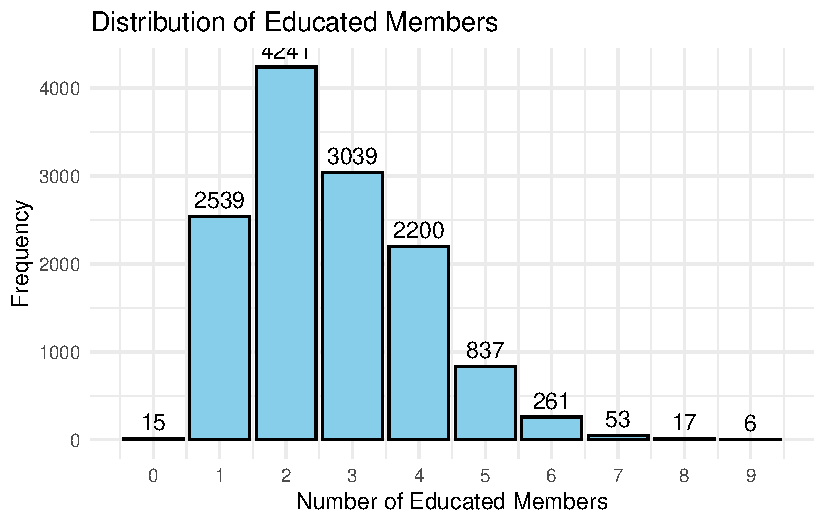
\includegraphics{vulnerability_files/figure-pdf/fig-hh-education-1.pdf}

}

\caption{\label{fig-hh-education}Households for each number of educated
members}

\end{figure}%

\subsection{Access to water}\label{access-to-water}

``When shocks hit, access to these services is an important determinant
of the impact of the shock on welfare. For example, with access to
improved drinking water, contaminated water from flooding and storms, or
lack of water due to drought has less of an impact. Nevertheless, it is
essential to acknowledge that the current indicator of access to
improved drinking water, often represented by covered wells in
low-income countries, may not sufficiently reflect susceptibility to
contamination during extreme events such as floods or droughts.
Therefore, there is a need for future work to refine this indicator by
considering a potentially higher threshold. Metrics such as ``improved
piped water'' can offer a more precise assessment of the infrastructure
safeguarding against water-related risks in the event of shocks.'' (Doan
et al. 2023)

We take note of this caveat and choose the threshold water supply system
installed in the dwelling and water system tap in the yard or vicinity
as counting towards this dimension from the possible options below:

\begin{enumerate}
\def\labelenumi{\arabic{enumi}.}
\tightlist
\item
  The water supply system installed in the dwelling
\item
  The water system tap in the yard or vicinity
\item
  The well in the yard or vicinity
\item
  Natural spring in the yard or vicinity
\item
  River, lake, spring, channel
\item
  Bought water
\item
  Other
\end{enumerate}

\begin{Shaded}
\begin{Highlighting}[]
\NormalTok{vulnerable\_water }\OtherTok{\textless{}{-}}\NormalTok{ poverty }\SpecialCharTok{|\textgreater{}} 
  \FunctionTok{select}\NormalTok{(UID, WaterSource) }\SpecialCharTok{|\textgreater{}} 
  \FunctionTok{mutate}\NormalTok{(}
    \AttributeTok{vulnerability\_water =} \FunctionTok{if\_else}\NormalTok{(}
\NormalTok{      WaterSource }\SpecialCharTok{\textless{}} \DecValTok{3}\NormalTok{, }\DecValTok{0}\NormalTok{, }\DecValTok{1}\NormalTok{)) }\SpecialCharTok{|\textgreater{}} 
  \FunctionTok{select}\NormalTok{(}\SpecialCharTok{{-}}\NormalTok{WaterSource)}

\CommentTok{\# We check the distribution}

\FunctionTok{as.data.frame}\NormalTok{(}\FunctionTok{table}\NormalTok{(vulnerable\_water}\SpecialCharTok{$}\NormalTok{vulnerability\_water)) }\SpecialCharTok{|\textgreater{}} 
  \FunctionTok{gt}\NormalTok{()}
\end{Highlighting}
\end{Shaded}

\begin{table}
\fontsize{12.0pt}{14.4pt}\selectfont
\begin{tabular*}{\linewidth}{@{\extracolsep{\fill}}cr}
\toprule
Var1 & Freq \\ 
\midrule\addlinespace[2.5pt]
0 & 10709 \\ 
1 & 2499 \\ 
\bottomrule
\end{tabular*}
\end{table}

\subsection{Access to electricity}\label{access-to-electricity}

``With access to electricity, households are more likely to have assets
such as fans that can help with heatwaves. A fuller discussion is
available in the World Bank's Lifelines report (Hallegatte et al, 2019).
Whilst not a final selection of assets and infrastructure that matter
for determining the initial loss of the shock, these measures provide a
good first estimate to stimulate discussion.'' (Doan et al. 2023)
Variable \texttt{q11\_3} from the poverty dataset is a dummy that
determines whether the household has access to electricity.

\begin{Shaded}
\begin{Highlighting}[]
\NormalTok{vulnerable\_electricity }\OtherTok{\textless{}{-}}\NormalTok{ poverty }\SpecialCharTok{|\textgreater{}} 
  \FunctionTok{select}\NormalTok{(UID, q11\_3) }\SpecialCharTok{|\textgreater{}} 
  \FunctionTok{mutate}\NormalTok{(}
    \AttributeTok{vulnerability\_electricity =} \FunctionTok{if\_else}\NormalTok{(}
\NormalTok{      q11\_3 }\SpecialCharTok{!=} \DecValTok{1}\NormalTok{, }\DecValTok{1}\NormalTok{, }\DecValTok{0}\NormalTok{)) }\SpecialCharTok{|\textgreater{}} 
  \FunctionTok{select}\NormalTok{(}\SpecialCharTok{{-}}\NormalTok{q11\_3)}

\CommentTok{\# We check the distribution}

\FunctionTok{as.data.frame}\NormalTok{(}\FunctionTok{table}\NormalTok{(vulnerable\_electricity}\SpecialCharTok{$}\NormalTok{vulnerability\_electricity)) }\SpecialCharTok{|\textgreater{}} 
  \FunctionTok{gt}\NormalTok{()}
\end{Highlighting}
\end{Shaded}

\begin{table}
\fontsize{12.0pt}{14.4pt}\selectfont
\begin{tabular*}{\linewidth}{@{\extracolsep{\fill}}cr}
\toprule
Var1 & Freq \\ 
\midrule\addlinespace[2.5pt]
0 & 13208 \\ 
\bottomrule
\end{tabular*}
\end{table}

Now, this is not a source of variation in the case of Georgia, since
100\% of households report having access to electricity, but the
methodology also mentions that ``Access to markets and services, access
to early warning systems, sanitation, and building and infrastructure
quality are also playing a key role in determining disasters' impacts,
and has been included in other estimates, but is left for future
inclusion here.'' (Doan et al. 2023). Both sanitation and building
infrastructure quality, proxied by wall materials could be included in
Georgia's estimates. When it comes to sanitation, there is still a gap
that the country needs to close.

\subsection{Access to sanitation}\label{access-to-sanitation}

For this variable (\texttt{TypeOfToilet}) we have the following
categories, of which we choose ``own flush toilet connected to the
sewerage system'' and ``shared flush toilet connected to the sewerage
system'' as having access to sanitation.

\begin{enumerate}
\def\labelenumi{\arabic{enumi}.}
\tightlist
\item
  Own flush toilet connected to the sewerage system
\item
  Shared flush toilet connected to the sewerage system
\item
  Flush latrine not connected to the sewerage system (connected to the
  river, chan
\item
  Pit latrine periodically cleaned or finally filled up and buried
\item
  Other
\end{enumerate}

\begin{Shaded}
\begin{Highlighting}[]
\NormalTok{vulnerable\_sanitation }\OtherTok{\textless{}{-}}\NormalTok{ poverty }\SpecialCharTok{|\textgreater{}} 
  \FunctionTok{select}\NormalTok{(UID, TypeOfToilet) }\SpecialCharTok{|\textgreater{}} 
  \FunctionTok{mutate}\NormalTok{(}
    \AttributeTok{vulnerability\_sanitation =} \FunctionTok{if\_else}\NormalTok{(}
\NormalTok{      TypeOfToilet }\SpecialCharTok{\textless{}} \DecValTok{3}\NormalTok{, }\DecValTok{0}\NormalTok{, }\DecValTok{1}\NormalTok{)) }\SpecialCharTok{|\textgreater{}} 
  \FunctionTok{select}\NormalTok{(}\SpecialCharTok{{-}}\NormalTok{TypeOfToilet)}

\CommentTok{\# We check the distribution}

\FunctionTok{as.data.frame}\NormalTok{(}\FunctionTok{table}\NormalTok{(vulnerable\_sanitation}\SpecialCharTok{$}\NormalTok{vulnerability\_sanitation)) }\SpecialCharTok{|\textgreater{}} 
  \FunctionTok{gt}\NormalTok{()}
\end{Highlighting}
\end{Shaded}

\begin{table}
\fontsize{12.0pt}{14.4pt}\selectfont
\begin{tabular*}{\linewidth}{@{\extracolsep{\fill}}cr}
\toprule
Var1 & Freq \\ 
\midrule\addlinespace[2.5pt]
0 & 5557 \\ 
1 & 7651 \\ 
\bottomrule
\end{tabular*}
\end{table}

\subsection{Building materials}\label{building-materials}

When it comes to building materials of walls and floor, data show that
the most precarious categories (mud walls, and bare ground floors) are
not present in the country. We will still count concrete walls as not
vulnerable and wood as vulnerable, but only relative to each other, not
making any assumptions about the quality of wood structures in Georgia.

\begin{Shaded}
\begin{Highlighting}[]
\NormalTok{vulnerable\_building }\OtherTok{\textless{}{-}}\NormalTok{ poverty }\SpecialCharTok{|\textgreater{}} 
  \FunctionTok{select}\NormalTok{(UID, Walls) }\SpecialCharTok{|\textgreater{}} 
  \FunctionTok{mutate}\NormalTok{(}
    \AttributeTok{vulnerability\_building =} \FunctionTok{if\_else}\NormalTok{(}
\NormalTok{      Walls }\SpecialCharTok{\%in\%} \FunctionTok{c}\NormalTok{(}\DecValTok{1}\NormalTok{,}\DecValTok{3}\NormalTok{), }\DecValTok{0}\NormalTok{, }\DecValTok{1}\NormalTok{)) }\SpecialCharTok{|\textgreater{}} 
  \FunctionTok{select}\NormalTok{(}\SpecialCharTok{{-}}\NormalTok{Walls)}

\CommentTok{\# We check the distribution}

\FunctionTok{as.data.frame}\NormalTok{(}\FunctionTok{table}\NormalTok{(}
\NormalTok{  vulnerable\_building}\SpecialCharTok{$}\NormalTok{vulnerability\_building)) }\SpecialCharTok{|\textgreater{}} 
  \FunctionTok{gt}\NormalTok{()}
\end{Highlighting}
\end{Shaded}

\begin{table}
\fontsize{12.0pt}{14.4pt}\selectfont
\begin{tabular*}{\linewidth}{@{\extracolsep{\fill}}cr}
\toprule
Var1 & Freq \\ 
\midrule\addlinespace[2.5pt]
0 & 11746 \\ 
1 & 1462 \\ 
\bottomrule
\end{tabular*}
\end{table}

\subsection{Social protection}\label{social-protection}

``The third dimension of inability to cope is access to public support.
There is considerable evidence that cash transfers help households to
manage shocks (\ldots) {[}T{]}here is some evidence in favor of using
information on current coverage, as support is more likely to be
available in response to a disaster in places where pre-disaster
coverage rates are high.'' (Doan et al. 2023) In the \texttt{poverty}
dataset the variable \texttt{S\_Q2b} shows those households that
actually received social protection benefits.

\begin{Shaded}
\begin{Highlighting}[]
\NormalTok{vulnerable\_ssp }\OtherTok{\textless{}{-}}\NormalTok{ poverty }\SpecialCharTok{|\textgreater{}} 
  \FunctionTok{select}\NormalTok{(UID, S\_Q2b) }\SpecialCharTok{|\textgreater{}} 
  \FunctionTok{mutate}\NormalTok{(}
    \AttributeTok{vulnerability\_ssp =} \FunctionTok{if\_else}\NormalTok{(}
      \FunctionTok{coalesce}\NormalTok{(S\_Q2b, }\DecValTok{0}\NormalTok{) }\SpecialCharTok{==} \DecValTok{1}\NormalTok{, }\DecValTok{0}\NormalTok{, }\DecValTok{1}\NormalTok{)) }\SpecialCharTok{|\textgreater{}} 
  \FunctionTok{select}\NormalTok{(}\SpecialCharTok{{-}}\NormalTok{S\_Q2b)}

\CommentTok{\# We check the distribution}

\FunctionTok{as.data.frame}\NormalTok{(}\FunctionTok{table}\NormalTok{(}
\NormalTok{  vulnerable\_ssp}\SpecialCharTok{$}\NormalTok{vulnerability\_ssp)) }\SpecialCharTok{|\textgreater{}} 
  \FunctionTok{gt}\NormalTok{()}
\end{Highlighting}
\end{Shaded}

\begin{table}
\fontsize{12.0pt}{14.4pt}\selectfont
\begin{tabular*}{\linewidth}{@{\extracolsep{\fill}}cr}
\toprule
Var1 & Freq \\ 
\midrule\addlinespace[2.5pt]
0 & 2330 \\ 
1 & 10878 \\ 
\bottomrule
\end{tabular*}
\end{table}

\subsection{Financial services}\label{financial-services}

``The variable we use indicates whether a respondent has either a
financial institution account or a mobile money account, given the
strong relationship in the literature on access to mobile money and
ability to use informal networks to manage the impact of large climate
shocks.'' (Doan et al. 2023) The \texttt{poverty} dataset has
information on amount saved by the household, which we will use as proxy
for access to some financial security. We cannot assert that the money
is being saved in a proper financial institution. However, we assume
that having monthly level of savings of any kind can mitigate the
impacts of climate change.

\begin{Shaded}
\begin{Highlighting}[]
\NormalTok{vulnerable\_financial }\OtherTok{\textless{}{-}}\NormalTok{ poverty }\SpecialCharTok{|\textgreater{}} 
  \FunctionTok{select}\NormalTok{(UID, DazogvaAnCasesxeba) }\SpecialCharTok{|\textgreater{}} 
  \FunctionTok{mutate}\NormalTok{(}
    \AttributeTok{vulnerability\_financial =} \FunctionTok{if\_else}\NormalTok{(}
      \FunctionTok{coalesce}\NormalTok{(DazogvaAnCasesxeba, }\DecValTok{0}\NormalTok{) }\SpecialCharTok{==} \DecValTok{0}\NormalTok{, }\DecValTok{1}\NormalTok{, }\DecValTok{0}\NormalTok{)) }\SpecialCharTok{|\textgreater{}} 
  \FunctionTok{select}\NormalTok{(}\SpecialCharTok{{-}}\NormalTok{DazogvaAnCasesxeba)}

\CommentTok{\# We check the distribution}

\FunctionTok{as.data.frame}\NormalTok{(}\FunctionTok{table}\NormalTok{(}
\NormalTok{  vulnerable\_financial}\SpecialCharTok{$}\NormalTok{vulnerability\_financial)) }\SpecialCharTok{|\textgreater{}} 
  \FunctionTok{gt}\NormalTok{()}
\end{Highlighting}
\end{Shaded}

\begin{table}
\fontsize{12.0pt}{14.4pt}\selectfont
\begin{tabular*}{\linewidth}{@{\extracolsep{\fill}}cr}
\toprule
Var1 & Freq \\ 
\midrule\addlinespace[2.5pt]
0 & 4777 \\ 
1 & 8431 \\ 
\bottomrule
\end{tabular*}
\end{table}

\subsection{Join vulnerability
datasets}\label{join-vulnerability-datasets}

\begin{Shaded}
\begin{Highlighting}[]
\CommentTok{\# List of data frames to join}
\NormalTok{vulnerable\_data }\OtherTok{\textless{}{-}} \FunctionTok{list}\NormalTok{(}
\NormalTok{  vulnerable\_education,}
\NormalTok{  vulnerable\_water,}
\NormalTok{  vulnerable\_electricity,}
\NormalTok{  vulnerable\_sanitation,}
\NormalTok{  vulnerable\_building,}
\NormalTok{  vulnerable\_ssp,}
\NormalTok{  vulnerable\_financial}
\NormalTok{)}

\CommentTok{\# Start with the initial data frame}
\ControlFlowTok{for}\NormalTok{ (df }\ControlFlowTok{in}\NormalTok{ vulnerable\_data) \{}
\NormalTok{  hh\_vulnerable }\OtherTok{\textless{}{-}}\NormalTok{ hh\_vulnerable }\SpecialCharTok{|\textgreater{}} \FunctionTok{left\_join}\NormalTok{(df, }\FunctionTok{join\_by}\NormalTok{(UID))}
\NormalTok{\}}
\end{Highlighting}
\end{Shaded}

\section{Exposure}\label{exposure}

Results are first presented for the number of people exposed to floods.
Exposure numbers are presented for a range of return periods (from 5 to
100) and using different intensity thresholds to define extreme events:
flood inundation of 15cm, 50cm and 150cm.

We first estimate the percentage of the population impacted by 1-in-100
year floods by region.

\begin{Shaded}
\begin{Highlighting}[]
\NormalTok{exposure\_pct }\OtherTok{\textless{}{-}}\NormalTok{ floods }\SpecialCharTok{|\textgreater{}} 
  \FunctionTok{mutate}\NormalTok{(}
    \AttributeTok{exposure\_pct =}\NormalTok{ exposure }\SpecialCharTok{/}\NormalTok{ total\_pop,}
    \AttributeTok{no\_exposure\_pct =} \DecValTok{1} \SpecialCharTok{{-}}\NormalTok{ exposure\_pct}
\NormalTok{  ) }\SpecialCharTok{|\textgreater{}} 
  \FunctionTok{filter}\NormalTok{(}
\NormalTok{    scenario }\SpecialCharTok{==} \StringTok{"2020"}
\NormalTok{  ) }\SpecialCharTok{|\textgreater{}} 
  \FunctionTok{select}\NormalTok{(}\FunctionTok{c}\NormalTok{(RegNo, regions, exposure\_pct, no\_exposure\_pct)) }\SpecialCharTok{|\textgreater{}} 
  \FunctionTok{arrange}\NormalTok{(RegNo)}

\NormalTok{exposure\_pct }\SpecialCharTok{|\textgreater{}} 
  \FunctionTok{gt}\NormalTok{()}
\end{Highlighting}
\end{Shaded}

\begin{table}

\caption{\label{tbl-exposure-pct}Exposure to floods percentage}

\centering{

\fontsize{12.0pt}{14.4pt}\selectfont
\begin{tabular*}{\linewidth}{@{\extracolsep{\fill}}rlrr}
\toprule
RegNo & regions & exposure\_pct & no\_exposure\_pct \\ 
\midrule\addlinespace[2.5pt]
0 & Kakheti & 0.02091671 & 0.9790833 \\ 
1 & Tbilisi & 0.07640243 & 0.9235976 \\ 
2 & Shida Kartli & 0.14236196 & 0.8576380 \\ 
3 & Kvemo Kartli & 0.04869128 & 0.9513087 \\ 
5 & Samtskhe-Javakheti & 0.12681053 & 0.8731895 \\ 
7 & Adjara Aut. Rep. & 0.06310201 & 0.9368980 \\ 
8 & Guria & 0.11072107 & 0.8892789 \\ 
9 & Samergelo and Zemo (upper) Svaneti & 0.15989061 & 0.8401094 \\ 
10 & Imereti & 0.10728398 & 0.8927160 \\ 
11 & Mtskheta-Mtianeti & 0.10345240 & 0.8965476 \\ 
12 & Abkhazia Aut. Rep. & 0.05764768 & 0.9423523 \\ 
13 & Racha-Lechkhumi and Kvemo (lower) Svaneti & 0.22102424 & 0.7789758 \\ 
\bottomrule
\end{tabular*}

}

\end{table}%

We then create subgroups based on adjustments to the weights column.

\begin{Shaded}
\begin{Highlighting}[]
\NormalTok{exposed }\OtherTok{\textless{}{-}}\NormalTok{ hh\_vulnerable }\SpecialCharTok{|\textgreater{}} 
  \FunctionTok{filter}\NormalTok{(QuartNo }\SpecialCharTok{==} \FunctionTok{unique}\NormalTok{(QuartNo)[}\DecValTok{1}\NormalTok{]) }\SpecialCharTok{|\textgreater{}} 
  \FunctionTok{left\_join}\NormalTok{(}
\NormalTok{    exposure\_pct, }
    \FunctionTok{join\_by}\NormalTok{(RegNo)) }\SpecialCharTok{|\textgreater{}} 
  \FunctionTok{mutate}\NormalTok{(}
    \AttributeTok{weights\_exposure =}\NormalTok{ weights\_quar }\SpecialCharTok{*}\NormalTok{ exposure\_pct,}
    \AttributeTok{exposed\_to\_floods =} \DecValTok{1}
\NormalTok{  ) }\SpecialCharTok{|\textgreater{}} 
  \FunctionTok{mutate}\NormalTok{(}
    \AttributeTok{exposed\_to\_floods =} \FunctionTok{factor}\NormalTok{(}
\NormalTok{      exposed\_to\_floods,}
      \AttributeTok{levels =} \FunctionTok{c}\NormalTok{(}\DecValTok{1}\NormalTok{, }\DecValTok{0}\NormalTok{),}
      \AttributeTok{labels =} \FunctionTok{c}\NormalTok{(}\StringTok{"Exposed"}\NormalTok{, }\StringTok{"Not exposed"}\NormalTok{)}
\NormalTok{    )}
\NormalTok{  )}

\NormalTok{not\_exposed }\OtherTok{\textless{}{-}}\NormalTok{ exposed }\SpecialCharTok{|\textgreater{}} 
  \FunctionTok{mutate}\NormalTok{(}
    \AttributeTok{weights\_exposure =}\NormalTok{ weights\_quar }\SpecialCharTok{*}\NormalTok{ no\_exposure\_pct,}
    \AttributeTok{exposed\_to\_floods =} \DecValTok{0}
\NormalTok{  ) }\SpecialCharTok{|\textgreater{}} 
  \FunctionTok{mutate}\NormalTok{(}
    \AttributeTok{exposed\_to\_floods =} \FunctionTok{factor}\NormalTok{(}
\NormalTok{      exposed\_to\_floods,}
      \AttributeTok{levels =} \FunctionTok{c}\NormalTok{(}\DecValTok{1}\NormalTok{, }\DecValTok{0}\NormalTok{),}
      \AttributeTok{labels =} \FunctionTok{c}\NormalTok{(}\StringTok{"Exposed"}\NormalTok{, }\StringTok{"Not exposed"}\NormalTok{)}
\NormalTok{    ))}

\NormalTok{vulnerable\_data }\OtherTok{\textless{}{-}} \FunctionTok{rbind}\NormalTok{(exposed, not\_exposed)}
\end{Highlighting}
\end{Shaded}

\section{Results}\label{results}

\subsection{Exposure to extreme weather events and
poverty}\label{exposure-to-extreme-weather-events-and-poverty}

We first replicate the paper's graph regarding exposure at different
return periods. Exposure numbers are presented for a range of return
periods (from 5 to 100) at one intensity threshold: flood inundation of
15cm, 50cm and 150cm. Exposure falls with the event severity and
increases with the return period.The figure shows that, given increasing
return periods, exposure will increase more dramatically at a 100 year
return period for Tbilisi (88,865 individuals), Imereti (53,027),
Samergeolo and Zemo (upper) Svaneti (48,964), and Shida Kartli (36,314).

\begin{Shaded}
\begin{Highlighting}[]
\NormalTok{floods\_all\_returns}\SpecialCharTok{$}\NormalTok{regions }\OtherTok{\textless{}{-}} \FunctionTok{factor}\NormalTok{(}
\NormalTok{  floods\_all\_returns}\SpecialCharTok{$}\NormalTok{regions,}
  \AttributeTok{levels =} \FunctionTok{unique}\NormalTok{(floods\_all\_returns}\SpecialCharTok{$}\NormalTok{regions)}
\NormalTok{)}

\NormalTok{floods\_all\_returns }\SpecialCharTok{|\textgreater{}} 
  \FunctionTok{filter}\NormalTok{(rt\_period }\SpecialCharTok{\textless{}} \DecValTok{200}\NormalTok{) }\SpecialCharTok{|\textgreater{}} 
  \FunctionTok{ggplot}\NormalTok{(}\FunctionTok{aes}\NormalTok{(}
    \AttributeTok{x =}\NormalTok{ rt\_period, }
    \AttributeTok{y =}\NormalTok{ exposure, }
    \AttributeTok{color =}\NormalTok{ regions)) }\SpecialCharTok{+}
  \FunctionTok{geom\_line}\NormalTok{(}\AttributeTok{size =} \DecValTok{1}\NormalTok{) }\SpecialCharTok{+}                      \CommentTok{\# Add lines for each region}
  \FunctionTok{geom\_point}\NormalTok{(}\AttributeTok{size =} \DecValTok{3}\NormalTok{) }\SpecialCharTok{+}                     \CommentTok{\# Add points for each region}
  \FunctionTok{scale\_color\_manual}\NormalTok{(}
    \AttributeTok{values =} \FunctionTok{c}\NormalTok{(}
      \StringTok{"yellow"}\NormalTok{,    }\StringTok{"darkblue"}\NormalTok{, }\StringTok{"orange"}\NormalTok{, }
      \StringTok{"gold"}\NormalTok{,      }\StringTok{"green"}\NormalTok{,    }\StringTok{"purple"}\NormalTok{, }
      \StringTok{"cyan"}\NormalTok{,      }\StringTok{"brown"}\NormalTok{,    }\StringTok{"pink"}\NormalTok{, }
      \StringTok{"darkgreen"}\NormalTok{, }\StringTok{"navy"}\NormalTok{,     }\StringTok{"red"}
\NormalTok{  )) }\SpecialCharTok{+}                                       \CommentTok{\# Provide enough colors for all regions}
  \FunctionTok{labs}\NormalTok{(}
    \AttributeTok{title =} \StringTok{"Flood exposure by return period"}\NormalTok{,}
    \AttributeTok{subtitle =} \StringTok{"Regions of Georgia"}\NormalTok{,}
    \AttributeTok{x =} \StringTok{"Return period (years)"}\NormalTok{,}
    \AttributeTok{y =} \StringTok{"Population exposed (individuals)"}
\NormalTok{  ) }\SpecialCharTok{+}
  \FunctionTok{theme\_minimal}\NormalTok{() }\SpecialCharTok{+}
  \FunctionTok{theme}\NormalTok{(}
    \AttributeTok{legend.title =} \FunctionTok{element\_blank}\NormalTok{(),          }\CommentTok{\# Remove legend title}
    \AttributeTok{legend.position =} \StringTok{"right"}                \CommentTok{\# Position legend on the right}
\NormalTok{  )}
\end{Highlighting}
\end{Shaded}

\begin{figure}[H]

\centering{

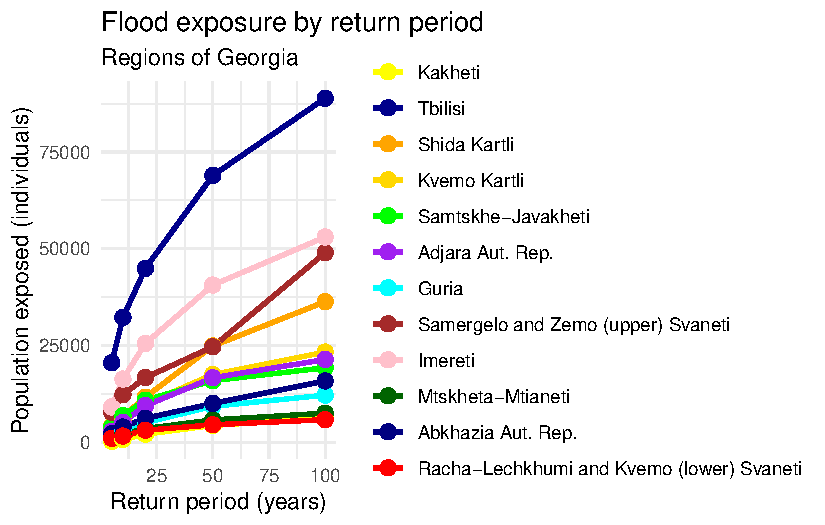
\includegraphics{vulnerability_files/figure-pdf/fig-floods-exposure-1.pdf}

}

\caption{\label{fig-floods-exposure}Georgia: Flood exposure by return
period and region}

\end{figure}%

\subsubsection{Extreme weather and poor by
region}\label{extreme-weather-and-poor-by-region}

We now turn to the question of those who are exposed and poor. We use
the official poverty line.

\begin{Shaded}
\begin{Highlighting}[]
\NormalTok{exposed\_and\_poor }\OtherTok{\textless{}{-}}\NormalTok{ vulnerable\_data }\SpecialCharTok{|\textgreater{}}
  \FunctionTok{mutate}\NormalTok{(}
    \AttributeTok{conspoor =} \FunctionTok{if\_else}\NormalTok{(}
\NormalTok{      aecons }\SpecialCharTok{\textless{}}\NormalTok{ pline, }\StringTok{"Below PL"}\NormalTok{, }\StringTok{"Above PL"}\NormalTok{),}
    \AttributeTok{individuals =}\NormalTok{ weights\_exposure }\SpecialCharTok{*}\NormalTok{ hhsize}
\NormalTok{  ) }\SpecialCharTok{|\textgreater{}} 
  \FunctionTok{group\_by}\NormalTok{(}\FunctionTok{as\_factor}\NormalTok{(RegNo), exposed\_to\_floods, conspoor) }\SpecialCharTok{|\textgreater{}} 
  \FunctionTok{summarize}\NormalTok{(}
    \AttributeTok{individuals =} \FunctionTok{sum}\NormalTok{(individuals, }\AttributeTok{na.rm =} \ConstantTok{TRUE}\NormalTok{)}
\NormalTok{  ) }\SpecialCharTok{|\textgreater{}} 
  \FunctionTok{pivot\_wider}\NormalTok{(}
    \AttributeTok{id\_cols =} \FunctionTok{c}\NormalTok{(}\StringTok{\textasciigrave{}}\AttributeTok{as\_factor(RegNo)}\StringTok{\textasciigrave{}}\NormalTok{),}
    \AttributeTok{names\_from =} \FunctionTok{c}\NormalTok{(exposed\_to\_floods, conspoor),}
    \AttributeTok{values\_from =}\NormalTok{ individuals,}
    \AttributeTok{names\_expand =} \ConstantTok{TRUE}
\NormalTok{  ) }\SpecialCharTok{|\textgreater{}} 
  \FunctionTok{mutate}\NormalTok{(}
    \AttributeTok{total\_population =} \FunctionTok{rowSums}\NormalTok{(}\FunctionTok{across}\NormalTok{(}\FunctionTok{c}\NormalTok{(}\DecValTok{1}\SpecialCharTok{:}\DecValTok{4}\NormalTok{)), }\AttributeTok{na.rm =} \ConstantTok{TRUE}\NormalTok{),}
    \AttributeTok{total\_exposed =} \FunctionTok{rowSums}\NormalTok{(}\FunctionTok{across}\NormalTok{(}\FunctionTok{starts\_with}\NormalTok{(}\StringTok{"Exposed\_"}\NormalTok{)), }\AttributeTok{na.rm =}\NormalTok{ T),}
    \AttributeTok{Pct\_exposed\_from\_total =}\NormalTok{ total\_exposed }\SpecialCharTok{/}\NormalTok{ total\_population }\SpecialCharTok{*} \DecValTok{100}\NormalTok{,}
    \AttributeTok{Pct\_below\_from\_exposed =} \StringTok{\textasciigrave{}}\AttributeTok{Exposed\_Below PL}\StringTok{\textasciigrave{}} \SpecialCharTok{/}\NormalTok{ total\_exposed }\SpecialCharTok{*}\DecValTok{100}
\NormalTok{  ) }\SpecialCharTok{|\textgreater{}} 
  \FunctionTok{select}\NormalTok{(}
    \StringTok{\textasciigrave{}}\AttributeTok{as\_factor(RegNo)}\StringTok{\textasciigrave{}}\NormalTok{,}
\NormalTok{    total\_population,}
\NormalTok{    total\_exposed,}
    \StringTok{\textasciigrave{}}\AttributeTok{Exposed\_Below PL}\StringTok{\textasciigrave{}}\NormalTok{,}
    \FunctionTok{starts\_with}\NormalTok{(}\StringTok{"Pct"}\NormalTok{)}
\NormalTok{  )}

\FunctionTok{names}\NormalTok{(exposed\_and\_poor) }\OtherTok{\textless{}{-}} \FunctionTok{c}\NormalTok{(}
  \StringTok{"Regions"}\NormalTok{,}
  \StringTok{"Total Population"}\NormalTok{,}
  \StringTok{"Total Exposed"}\NormalTok{,}
  \StringTok{"Exposed Below PL"}\NormalTok{,}
  \StringTok{"Pct. exposed from total"}\NormalTok{,}
  \StringTok{"Pct. Below PL from exposed"}
\NormalTok{)}

\NormalTok{exposed\_and\_poor }\SpecialCharTok{|\textgreater{}} 
  \FunctionTok{ungroup}\NormalTok{() }\SpecialCharTok{|\textgreater{}} 
  \FunctionTok{gt}\NormalTok{() }\SpecialCharTok{|\textgreater{}} 
  \FunctionTok{fmt\_number}\NormalTok{(}
    \AttributeTok{columns =} \FunctionTok{c}\NormalTok{(}\DecValTok{2}\SpecialCharTok{:}\DecValTok{4}\NormalTok{),   }\CommentTok{\# Apply formatting to totals columns}
    \AttributeTok{decimals =} \DecValTok{0}\NormalTok{,                 }\CommentTok{\# Set no decimals}
    \AttributeTok{use\_seps =} \ConstantTok{TRUE}               \CommentTok{\# Use thousands separator}
\NormalTok{  ) }\SpecialCharTok{|\textgreater{}} 
  \FunctionTok{fmt\_number}\NormalTok{(}
    \AttributeTok{columns =} \FunctionTok{c}\NormalTok{(}\DecValTok{5}\SpecialCharTok{:}\DecValTok{6}\NormalTok{),   }\CommentTok{\# Apply formatting to percent columns}
    \AttributeTok{decimals =} \DecValTok{1}                 \CommentTok{\# Set one decimal}
\NormalTok{  )}
\end{Highlighting}
\end{Shaded}

\begin{table}

\caption{\label{tbl-exposure-dataset}Number of people exposed to extreme
weather and poor}

\centering{

\fontsize{12.0pt}{14.4pt}\selectfont
\begin{tabular*}{\linewidth}{@{\extracolsep{\fill}}crrrrr}
\toprule
Region & Total Population & Total Exposed & Exposed Below PL & Pct. exposed from total & Pct. Below PL from exposed \\ 
\midrule\addlinespace[2.5pt]
Kakheti & 307,650 & 6,435 & 477 & 2.1 & 7.4 \\ 
Tbilisi & 1,206,504 & 92,180 & 5,067 & 7.6 & 5.5 \\ 
Shida Kartli & 251,397 & 35,789 & 4,667 & 14.2 & 13.0 \\ 
Kvemo Kartli & 454,698 & 22,140 & 4,077 & 4.9 & 18.4 \\ 
Samtskhe-Javakheti & 150,422 & 19,075 & 2,120 & 12.7 & 11.1 \\ 
Adjara A.R. & 370,642 & 23,388 & 3,902 & 6.3 & 16.7 \\ 
Guria & 104,588 & 11,580 & 2,932 & 11.1 & 25.3 \\ 
Samegrelo-Zemo Svaneti & 285,438 & 45,639 & 7,934 & 16.0 & 17.4 \\ 
Imereti & 459,035 & 49,247 & 4,905 & 10.7 & 10.0 \\ 
Mtskheta-Mtianeti & 95,389 & 9,868 & 1,549 & 10.3 & 15.7 \\ 
Racha-Lechkhumi and Kvemo Svaneti & 28,113 & 6,214 & 879 & 22.1 & 14.1 \\ 
\bottomrule
\end{tabular*}

}

\end{table}%

\subsubsection{Extreme weather and poor by consumption
quintile}\label{extreme-weather-and-poor-by-consumption-quintile}

The paper replicates the table by country income level. Since our tables
are at the country level, we could replicate these results by income
(consumption) quintile, but as evident below it is a rather
uninformative table, because those below poverty belong exclusively to
the first quintile, leaving the remaining of the table unpopulated.

\begin{Shaded}
\begin{Highlighting}[]
\NormalTok{exposed\_and\_poor\_q }\OtherTok{\textless{}{-}}\NormalTok{ vulnerable\_data }\SpecialCharTok{|\textgreater{}}
  \FunctionTok{mutate}\NormalTok{(}
    \AttributeTok{conspoor =} \FunctionTok{if\_else}\NormalTok{(}
\NormalTok{      aecons }\SpecialCharTok{\textless{}}\NormalTok{ pline, }\StringTok{"Below PL"}\NormalTok{, }\StringTok{"Above PL"}\NormalTok{),}
    \AttributeTok{individuals =}\NormalTok{ weights\_exposure }\SpecialCharTok{*}\NormalTok{ hhsize}
\NormalTok{  ) }\SpecialCharTok{|\textgreater{}} 
  \FunctionTok{group\_by}\NormalTok{(quintilc, exposed\_to\_floods, conspoor) }\SpecialCharTok{|\textgreater{}} 
  \FunctionTok{summarize}\NormalTok{(}
    \AttributeTok{individuals =} \FunctionTok{sum}\NormalTok{(}\FunctionTok{coalesce}\NormalTok{(individuals,}\DecValTok{0}\NormalTok{), }\AttributeTok{na.rm =} \ConstantTok{TRUE}\NormalTok{)}
\NormalTok{  ) }\SpecialCharTok{|\textgreater{}} 
  \FunctionTok{pivot\_wider}\NormalTok{(}
    \AttributeTok{id\_cols =} \FunctionTok{c}\NormalTok{(quintilc),}
    \AttributeTok{names\_from =} \FunctionTok{c}\NormalTok{(exposed\_to\_floods, conspoor),}
    \AttributeTok{values\_from =}\NormalTok{ individuals,}
    \AttributeTok{names\_expand =} \ConstantTok{TRUE}\NormalTok{,}
    \AttributeTok{values\_fill =} \DecValTok{0}
\NormalTok{  ) }\SpecialCharTok{|\textgreater{}} 
  \FunctionTok{mutate}\NormalTok{(}
    \AttributeTok{total\_population =} \FunctionTok{rowSums}\NormalTok{(}\FunctionTok{across}\NormalTok{(}\FunctionTok{c}\NormalTok{(}\DecValTok{1}\SpecialCharTok{:}\DecValTok{4}\NormalTok{)), }\AttributeTok{na.rm =} \ConstantTok{TRUE}\NormalTok{),}
    \AttributeTok{total\_exposed =} \FunctionTok{rowSums}\NormalTok{(}\FunctionTok{across}\NormalTok{(}\FunctionTok{starts\_with}\NormalTok{(}\StringTok{"Exposed\_"}\NormalTok{)), }\AttributeTok{na.rm =}\NormalTok{ T),}
    \AttributeTok{Pct\_exposed\_from\_total =}\NormalTok{ total\_exposed }\SpecialCharTok{/}\NormalTok{ total\_population }\SpecialCharTok{*} \DecValTok{100}\NormalTok{,}
    \AttributeTok{Pct\_below\_from\_exposed =} \StringTok{\textasciigrave{}}\AttributeTok{Exposed\_Below PL}\StringTok{\textasciigrave{}} \SpecialCharTok{/}\NormalTok{ total\_exposed }\SpecialCharTok{*}\DecValTok{100}
\NormalTok{  ) }\SpecialCharTok{|\textgreater{}} 
  \FunctionTok{select}\NormalTok{(}
\NormalTok{    quintilc,}
\NormalTok{    total\_population,}
\NormalTok{    total\_exposed,}
    \StringTok{\textasciigrave{}}\AttributeTok{Exposed\_Below PL}\StringTok{\textasciigrave{}}\NormalTok{,}
    \FunctionTok{starts\_with}\NormalTok{(}\StringTok{"Pct"}\NormalTok{)}
\NormalTok{  ) }\SpecialCharTok{|\textgreater{}} 
  \FunctionTok{ungroup}\NormalTok{()}

\FunctionTok{colnames}\NormalTok{(exposed\_and\_poor\_q) }\OtherTok{\textless{}{-}} \FunctionTok{c}\NormalTok{(}
  \StringTok{"Quintiles"}\NormalTok{,}
  \StringTok{"Total Population"}\NormalTok{,}
  \StringTok{"Total Exposed"}\NormalTok{,}
  \StringTok{"Exposed Below PL"}\NormalTok{,}
  \StringTok{"Pct. exposed from total"}\NormalTok{,}
  \StringTok{"Pct. Below PL from exposed"}
\NormalTok{)}

\NormalTok{exposed\_and\_poor\_q }\SpecialCharTok{|\textgreater{}} 
  \FunctionTok{gt}\NormalTok{() }\SpecialCharTok{|\textgreater{}} 
  \FunctionTok{fmt\_number}\NormalTok{(}
    \AttributeTok{columns =} \FunctionTok{c}\NormalTok{(}\DecValTok{2}\SpecialCharTok{:}\DecValTok{4}\NormalTok{),   }\CommentTok{\# Apply formatting to totals columns}
    \AttributeTok{decimals =} \DecValTok{0}\NormalTok{,                 }\CommentTok{\# Set no decimals}
    \AttributeTok{use\_seps =} \ConstantTok{TRUE}               \CommentTok{\# Use thousands separator}
\NormalTok{  ) }\SpecialCharTok{|\textgreater{}} 
  \FunctionTok{fmt\_number}\NormalTok{(}
    \AttributeTok{columns =} \FunctionTok{c}\NormalTok{(}\DecValTok{5}\SpecialCharTok{:}\DecValTok{6}\NormalTok{),   }\CommentTok{\# Apply formatting to percent columns}
    \AttributeTok{decimals =} \DecValTok{1}                 \CommentTok{\# Set one decimal}
\NormalTok{  )}
\end{Highlighting}
\end{Shaded}

\begin{table}

\caption{\label{tbl-exposure-quintile}Number of people exposed to
extreme weather and poor}

\centering{

\fontsize{12.0pt}{14.4pt}\selectfont
\begin{tabular*}{\linewidth}{@{\extracolsep{\fill}}rrrrrr}
\toprule
Quintiles of aecons & Total Population & Total Exposed & Exposed Below PL & Pct. exposed from total & Pct. Below PL from exposed \\ 
\midrule\addlinespace[2.5pt]
1 & 676,026 & 60,685 & 38,508 & 9.0 & 63.5 \\ 
2 & 826,458 & 69,537 & 0 & 8.4 & 0.0 \\ 
3 & 787,172 & 68,020 & 0 & 8.6 & 0.0 \\ 
4 & 721,889 & 61,521 & 0 & 8.5 & 0.0 \\ 
5 & 702,330 & 61,793 & 0 & 8.8 & 0.0 \\ 
\bottomrule
\end{tabular*}

}

\end{table}%

\subsection{At risk from extreme weather
events}\label{at-risk-from-extreme-weather-events}

\subsubsection{Number of people exposed and vulnerable in each
indicator}\label{number-of-people-exposed-and-vulnerable-in-each-indicator}

``For these same events and risk thresholds, we consider the share of
households that are exposed and highly vulnerable. Being highly
vulnerable is defined as failing to reach the threshold in or lacking
access to one or more dimensions (e.g., lacking access to electricity or
coverage by social protection or having an insufficient income).'' (Doan
et al. 2023)

\begin{Shaded}
\begin{Highlighting}[]
\NormalTok{at\_risk }\OtherTok{\textless{}{-}}\NormalTok{ vulnerable\_data }\SpecialCharTok{|\textgreater{}}
  \FunctionTok{mutate}\NormalTok{(}
    \AttributeTok{conspoor =} \FunctionTok{if\_else}\NormalTok{(}
\NormalTok{      aecons }\SpecialCharTok{\textless{}}\NormalTok{ pline, }\StringTok{"Below PL"}\NormalTok{, }\StringTok{"Above PL"}\NormalTok{),}
    \AttributeTok{individuals =}\NormalTok{ weights\_exposure }\SpecialCharTok{*}\NormalTok{ hhsize,}
    \AttributeTok{risk\_income =}\NormalTok{ individuals }\SpecialCharTok{*}\NormalTok{ vulnerability\_income,}
    \AttributeTok{risk\_education =}\NormalTok{ individuals }\SpecialCharTok{*}\NormalTok{ vulnerability\_education,}
    \AttributeTok{risk\_water =}\NormalTok{ individuals }\SpecialCharTok{*}\NormalTok{ vulnerability\_water,}
    \CommentTok{\# risk\_electricity = individuals * vulnerability\_electricity, \# 100\% in GEO}
    \AttributeTok{risk\_sanitation =}\NormalTok{ individuals }\SpecialCharTok{*}\NormalTok{ vulnerability\_sanitation,}
    \AttributeTok{risk\_building =}\NormalTok{ individuals }\SpecialCharTok{*}\NormalTok{ vulnerability\_building,}
    \AttributeTok{risk\_ssp =}\NormalTok{ individuals }\SpecialCharTok{*}\NormalTok{ vulnerability\_ssp,}
    \AttributeTok{risk\_financial =}\NormalTok{ individuals }\SpecialCharTok{*}\NormalTok{ vulnerability\_financial}
\NormalTok{  ) }\SpecialCharTok{|\textgreater{}} 
  \FunctionTok{group\_by}\NormalTok{(}\FunctionTok{as\_factor}\NormalTok{(RegNo), exposed\_to\_floods) }\SpecialCharTok{|\textgreater{}} 
  \FunctionTok{summarize}\NormalTok{(}
    \AttributeTok{Individuals =} \FunctionTok{sum}\NormalTok{(individuals, }\AttributeTok{na.rm =}\NormalTok{ T),}
    \AttributeTok{Income =} \FunctionTok{sum}\NormalTok{(risk\_income, }\AttributeTok{na.rm =}\NormalTok{ T),}
    \AttributeTok{Education =} \FunctionTok{sum}\NormalTok{(risk\_education, }\AttributeTok{na.rm =}\NormalTok{ T),}
    \AttributeTok{Water =} \FunctionTok{sum}\NormalTok{(risk\_water, }\AttributeTok{na.rm =}\NormalTok{ T),}
    \CommentTok{\# Electricity = sum(risk\_income, na.rm = T),}
    \AttributeTok{Sanitation =} \FunctionTok{sum}\NormalTok{(risk\_sanitation, }\AttributeTok{na.rm =}\NormalTok{ T),}
    \AttributeTok{Buildings =} \FunctionTok{sum}\NormalTok{(risk\_building, }\AttributeTok{na.rm =}\NormalTok{ T),}
    \AttributeTok{SSP =} \FunctionTok{sum}\NormalTok{(risk\_ssp, }\AttributeTok{na.rm =}\NormalTok{ T),}
    \AttributeTok{Financial =} \FunctionTok{sum}\NormalTok{(risk\_financial, }\AttributeTok{na.rm =}\NormalTok{ T)}
\NormalTok{  ) }\SpecialCharTok{|\textgreater{}} 
  \FunctionTok{pivot\_wider}\NormalTok{(}
    \AttributeTok{id\_cols =} \FunctionTok{c}\NormalTok{(}\StringTok{\textasciigrave{}}\AttributeTok{as\_factor(RegNo)}\StringTok{\textasciigrave{}}\NormalTok{),}
    \AttributeTok{names\_from =} \FunctionTok{c}\NormalTok{(exposed\_to\_floods),}
    \AttributeTok{values\_from =} \FunctionTok{c}\NormalTok{(}
\NormalTok{      Individuals,}
\NormalTok{      Income,}
\NormalTok{      Education,}
\NormalTok{      Water,}
      \CommentTok{\# Electricity,}
\NormalTok{      Sanitation,}
\NormalTok{      Buildings,}
\NormalTok{      SSP,}
\NormalTok{      Financial),}
    \AttributeTok{names\_expand =} \ConstantTok{TRUE}
\NormalTok{  ) }\SpecialCharTok{|\textgreater{}} 
  \FunctionTok{mutate}\NormalTok{(}
    \AttributeTok{total\_population =} \FunctionTok{rowSums}\NormalTok{(}\FunctionTok{across}\NormalTok{(}\FunctionTok{starts\_with}\NormalTok{(}\StringTok{"Individuals\_"}\NormalTok{)), }\AttributeTok{na.rm =} \ConstantTok{TRUE}\NormalTok{),}
\NormalTok{  ) }\SpecialCharTok{|\textgreater{}} 
  \FunctionTok{select}\NormalTok{(}
    \StringTok{\textasciigrave{}}\AttributeTok{as\_factor(RegNo)}\StringTok{\textasciigrave{}}\NormalTok{,}
\NormalTok{    total\_population,}
    \FunctionTok{ends\_with}\NormalTok{(}\StringTok{"\_Exposed"}\NormalTok{)}
\NormalTok{  ) }\SpecialCharTok{|\textgreater{}} 
  \FunctionTok{ungroup}\NormalTok{()}

\FunctionTok{names}\NormalTok{(at\_risk) }\OtherTok{\textless{}{-}} \FunctionTok{c}\NormalTok{(}
  \StringTok{"Regions"}\NormalTok{,}
  \StringTok{"Total Population"}\NormalTok{,}
  \StringTok{"Total Exposed"}\NormalTok{,}
  \StringTok{"Income"}\NormalTok{,}
  \StringTok{"Education"}\NormalTok{,}
  \StringTok{"Water"}\NormalTok{,}
  \StringTok{"Sanitation"}\NormalTok{,}
  \StringTok{"Buildings"}\NormalTok{,}
  \StringTok{"Social Protection"}\NormalTok{,}
  \StringTok{"Financial inclusion"}
\NormalTok{)}

\NormalTok{at\_risk }\SpecialCharTok{|\textgreater{}} 
  \FunctionTok{ungroup}\NormalTok{() }\SpecialCharTok{|\textgreater{}} 
  \FunctionTok{gt}\NormalTok{() }\SpecialCharTok{|\textgreater{}} 
  \FunctionTok{fmt\_number}\NormalTok{(}
    \AttributeTok{columns =} \FunctionTok{where}\NormalTok{(is.numeric),   }\CommentTok{\# Apply formatting to totals columns}
    \AttributeTok{decimals =} \DecValTok{0}\NormalTok{,                 }\CommentTok{\# Set no decimals}
    \AttributeTok{use\_seps =} \ConstantTok{TRUE}               \CommentTok{\# Use thousands separator}
\NormalTok{  )}
\CommentTok{\# write.table(at\_risk, "clipboard", sep = "\textbackslash{}t", row.names = F)}
\end{Highlighting}
\end{Shaded}

\begin{table}

\caption{\label{tbl-at-risk-region}Number of people exposed and
vulnerable by region}

\centering{

\fontsize{12.0pt}{14.4pt}\selectfont
\begin{tabular*}{\linewidth}{@{\extracolsep{\fill}}crrrrrrrrr}
\toprule
Region & Total Population & Total Exposed & Income & Education & Water & Sanitation & Buildings & Social Protection & Financial inclusion \\ 
\midrule\addlinespace[2.5pt]
Kakheti & 307,650 & 6,435 & 1,462 & 0 & 1,344 & 5,500 & 0 & 5,562 & 3,816 \\ 
Tbilisi & 1,206,504 & 92,180 & 22,275 & 0 & 0 & 351 & 417 & 78,230 & 61,190 \\ 
Shida Kartli & 251,397 & 35,789 & 10,725 & 51 & 9,154 & 19,837 & 480 & 29,582 & 19,092 \\ 
Kvemo Kartli & 454,698 & 22,140 & 9,866 & 187 & 1,608 & 12,548 & 895 & 17,200 & 16,079 \\ 
Samtskhe-Javakheti & 150,422 & 19,075 & 4,545 & 0 & 527 & 10,792 & 711 & 17,322 & 8,935 \\ 
Adjara A.R. & 370,642 & 23,388 & 9,368 & 0 & 3,601 & 8,754 & 3,259 & 19,401 & 11,569 \\ 
Guria & 104,588 & 11,580 & 6,547 & 0 & 4,836 & 8,391 & 4,119 & 9,425 & 7,691 \\ 
Samegrelo-Zemo Svaneti & 285,438 & 45,639 & 17,925 & 0 & 25,669 & 34,630 & 10,065 & 37,740 & 30,110 \\ 
Imereti & 459,035 & 49,247 & 10,541 & 0 & 14,325 & 24,106 & 2,647 & 38,173 & 23,016 \\ 
Mtskheta-Mtianeti & 95,389 & 9,868 & 3,945 & 11 & 424 & 5,634 & 22 & 8,680 & 6,632 \\ 
Racha-Lechkhumi and Kvemo Svaneti & 28,113 & 6,214 & 1,757 & 0 & 573 & 3,726 & 1,785 & 3,385 & 3,486 \\ 
\bottomrule
\end{tabular*}

}

\end{table}%

\subsubsection{Number of people highly vulnerable on multiple
dimensions}\label{number-of-people-highly-vulnerable-on-multiple-dimensions}

\begin{Shaded}
\begin{Highlighting}[]
\NormalTok{at\_risk\_dimensions }\OtherTok{\textless{}{-}}\NormalTok{ vulnerable\_data }\SpecialCharTok{|\textgreater{}}
  \FunctionTok{mutate}\NormalTok{(}
    \AttributeTok{individuals =}\NormalTok{ weights\_exposure }\SpecialCharTok{*}\NormalTok{ hhsize,}
    \AttributeTok{number\_of\_dimensions =} \FunctionTok{rowSums}\NormalTok{(}\FunctionTok{across}\NormalTok{(}\FunctionTok{starts\_with}\NormalTok{(}\StringTok{"vulnerability\_"}\NormalTok{)))}
\NormalTok{    ) }\SpecialCharTok{|\textgreater{}} 
  \FunctionTok{group\_by}\NormalTok{(}
    \FunctionTok{as\_factor}\NormalTok{(RegNo), }
\NormalTok{    exposed\_to\_floods, }
\NormalTok{    number\_of\_dimensions) }\SpecialCharTok{|\textgreater{}} 
  \FunctionTok{summarize}\NormalTok{(}
    \AttributeTok{Individuals =} \FunctionTok{sum}\NormalTok{(individuals, }\AttributeTok{na.rm =}\NormalTok{ T),}
\NormalTok{  ) }\SpecialCharTok{|\textgreater{}} 
  \FunctionTok{pivot\_wider}\NormalTok{(}
    \AttributeTok{id\_cols =} \FunctionTok{c}\NormalTok{(}\StringTok{\textasciigrave{}}\AttributeTok{as\_factor(RegNo)}\StringTok{\textasciigrave{}}\NormalTok{),}
    \AttributeTok{names\_from =} \FunctionTok{c}\NormalTok{(exposed\_to\_floods, number\_of\_dimensions),}
    \AttributeTok{values\_from =} \FunctionTok{c}\NormalTok{(}
\NormalTok{      Individuals),}
    \AttributeTok{names\_expand =} \ConstantTok{TRUE}\NormalTok{,}
    \AttributeTok{values\_fill =} \DecValTok{0}
\NormalTok{  ) }\SpecialCharTok{|\textgreater{}} 
  \FunctionTok{mutate}\NormalTok{(}
    \AttributeTok{total\_population =} \FunctionTok{rowSums}\NormalTok{(}\FunctionTok{across}\NormalTok{(}\FunctionTok{where}\NormalTok{(is.numeric)), }\AttributeTok{na.rm =} \ConstantTok{TRUE}\NormalTok{),}
    \AttributeTok{total\_exposed =} \FunctionTok{rowSums}\NormalTok{(}\FunctionTok{across}\NormalTok{(}\FunctionTok{starts\_with}\NormalTok{(}\StringTok{"Exposed\_"}\NormalTok{)), }\AttributeTok{na.rm =} \ConstantTok{TRUE}\NormalTok{)}
\NormalTok{  ) }\SpecialCharTok{|\textgreater{}} 
  \FunctionTok{select}\NormalTok{(}
    \StringTok{\textasciigrave{}}\AttributeTok{as\_factor(RegNo)}\StringTok{\textasciigrave{}}\NormalTok{,}
\NormalTok{    total\_population,}
\NormalTok{    total\_exposed,}
    \FunctionTok{starts\_with}\NormalTok{(}\StringTok{"Exposed\_"}\NormalTok{)}
\NormalTok{  ) }\SpecialCharTok{|\textgreater{}} 
  \FunctionTok{ungroup}\NormalTok{()}

\FunctionTok{names}\NormalTok{(at\_risk\_dimensions) }\OtherTok{\textless{}{-}} \FunctionTok{c}\NormalTok{(}
  \StringTok{"Regions"}\NormalTok{,}
  \StringTok{"Total Population"}\NormalTok{,}
  \StringTok{"Total Exposed"}\NormalTok{,}
  \StringTok{"0 dimensions"}\NormalTok{,}
  \StringTok{"1 dimension"}\NormalTok{,}
  \StringTok{"2 dimensions"}\NormalTok{,}
  \StringTok{"3 dimensions"}\NormalTok{,}
  \StringTok{"4 dimensions"}\NormalTok{,}
  \StringTok{"5 dimensions"}\NormalTok{,}
  \StringTok{"6 dimensions"}
\NormalTok{)}

\NormalTok{at\_risk\_dimensions }\SpecialCharTok{|\textgreater{}} 
  \FunctionTok{gt}\NormalTok{() }\SpecialCharTok{|\textgreater{}} 
  \FunctionTok{fmt\_number}\NormalTok{(}
    \AttributeTok{columns =} \FunctionTok{where}\NormalTok{(is.numeric),   }\CommentTok{\# Apply formatting to totals columns}
    \AttributeTok{decimals =} \DecValTok{0}\NormalTok{,                 }\CommentTok{\# Set no decimals}
    \AttributeTok{use\_seps =} \ConstantTok{TRUE}               \CommentTok{\# Use thousands separator}
\NormalTok{  )}
\CommentTok{\# write.table(at\_risk\_dimensions, "clipboard", sep = "\textbackslash{}t", row.names = F)}
\end{Highlighting}
\end{Shaded}

\begin{table}

\caption{\label{tbl-at-risk-dimensions}Number of people highly
vulnerable on multiple dimensions}

\centering{

\fontsize{12.0pt}{14.4pt}\selectfont
\begin{tabular*}{\linewidth}{@{\extracolsep{\fill}}crrrrrrrrr}
\toprule
Region & Total Population & Total Exposed & 0 dimensions & 1 dimension & 2 dimensions & 3 dimensions & 4 dimensions & 5 dimensions & 6 dimensions \\ 
\midrule\addlinespace[2.5pt]
Kakheti & 307,650 & 6,435 & 0 & 555 & 1,926 & 2,593 & 1,306 & 55 & 0 \\ 
Tbilisi & 1,206,504 & 92,180 & 2,088 & 28,552 & 50,877 & 10,496 & 167 & 0 & 0 \\ 
Shida Kartli & 251,397 & 35,789 & 50 & 7,054 & 10,963 & 12,153 & 4,393 & 1,152 & 26 \\ 
Kvemo Kartli & 454,698 & 22,140 & 155 & 3,449 & 6,095 & 7,320 & 4,821 & 300 & 0 \\ 
Samtskhe-Javakheti & 150,422 & 19,075 & 0 & 2,960 & 9,497 & 5,687 & 836 & 94 & 0 \\ 
Adjara A.R. & 370,642 & 23,388 & 123 & 5,746 & 8,252 & 5,136 & 2,584 & 1,322 & 224 \\ 
Guria & 104,588 & 11,580 & 15 & 632 & 2,365 & 2,105 & 3,469 & 2,511 & 484 \\ 
Samegrelo-Zemo Svaneti & 285,438 & 45,639 & 0 & 3,506 & 8,984 & 9,278 & 13,657 & 9,083 & 1,132 \\ 
Imereti & 459,035 & 49,247 & 1,871 & 13,060 & 13,742 & 11,645 & 7,315 & 1,614 & 0 \\ 
Mtskheta-Mtianeti & 95,389 & 9,868 & 102 & 1,853 & 2,374 & 3,657 & 1,631 & 250 & 0 \\ 
Racha-Lechkhumi and Kvemo Svaneti & 28,113 & 6,214 & 189 & 1,398 & 1,981 & 1,621 & 719 & 220 & 86 \\ 
\bottomrule
\end{tabular*}

}

\end{table}%

\subsubsection{Traditionally vulnerable
groups}\label{traditionally-vulnerable-groups}

\begin{Shaded}
\begin{Highlighting}[]
\NormalTok{traditionally\_vulnerable }\OtherTok{\textless{}{-}}\NormalTok{ vulnerable\_data }\SpecialCharTok{|\textgreater{}}
  \FunctionTok{mutate}\NormalTok{(}
    \AttributeTok{all\_members =}\NormalTok{ weights\_exposure }\SpecialCharTok{*}\NormalTok{ hhsize,}
    \AttributeTok{children =}\NormalTok{ weights\_exposure }\SpecialCharTok{*}\NormalTok{ Childern,}
    \AttributeTok{youth =}\NormalTok{ weights\_exposure }\SpecialCharTok{*}\NormalTok{ Adult,}
    \AttributeTok{women =}\NormalTok{ weights\_exposure }\SpecialCharTok{*}\NormalTok{ Working\_age\_Woman,}
    \AttributeTok{men =}\NormalTok{ weights\_exposure }\SpecialCharTok{*}\NormalTok{ Working\_age\_man,}
    \AttributeTok{elderly =}\NormalTok{ weights\_exposure }\SpecialCharTok{*}
\NormalTok{      (Pensioner\_age\_man }\SpecialCharTok{+}\NormalTok{ Pensioner\_age\_Woman)}
\NormalTok{  ) }\SpecialCharTok{|\textgreater{}}
  \FunctionTok{select}\NormalTok{(}
\NormalTok{    UID,}
\NormalTok{    RegNo,}
\NormalTok{    type,}
    \CommentTok{\# all\_members,}
\NormalTok{    children,}
\NormalTok{    youth,}
\NormalTok{    women,}
\NormalTok{    elderly,}
\NormalTok{    men,}
\NormalTok{    vulnerability\_income,}
\NormalTok{    vulnerability\_education,}
\NormalTok{    vulnerability\_water,}
\NormalTok{    vulnerability\_sanitation,}
\NormalTok{    vulnerability\_building,}
\NormalTok{    vulnerability\_ssp,}
\NormalTok{    vulnerability\_financial,}
\NormalTok{    exposed\_to\_floods}
\NormalTok{  ) }\SpecialCharTok{|\textgreater{}}
  \FunctionTok{pivot\_longer}\NormalTok{(}
    \AttributeTok{cols =} \FunctionTok{starts\_with}\NormalTok{(}\StringTok{"vulnerability\_"}\NormalTok{),}
    \AttributeTok{names\_to =} \StringTok{"vulnerability\_type"}\NormalTok{,}
    \AttributeTok{names\_prefix =} \StringTok{"vulnerability\_"}\NormalTok{,}
    \AttributeTok{values\_to =} \StringTok{"is\_vulnerable"}
\NormalTok{  ) }\SpecialCharTok{|\textgreater{}}
  \FunctionTok{pivot\_longer}\NormalTok{(}
    \AttributeTok{cols =} \FunctionTok{c}\NormalTok{(children, youth, women, elderly, men),}
    \AttributeTok{names\_to =} \StringTok{"vulnerable\_group"}\NormalTok{,}
    \AttributeTok{values\_to =} \StringTok{"no\_vulnerable\_people"}
\NormalTok{  ) }\SpecialCharTok{|\textgreater{}}
  \FunctionTok{filter}\NormalTok{(is\_vulnerable }\SpecialCharTok{==} \DecValTok{1}\NormalTok{, exposed\_to\_floods }\SpecialCharTok{==} \StringTok{"Exposed"}\NormalTok{) }\SpecialCharTok{|\textgreater{}}
  \FunctionTok{mutate}\NormalTok{(}
    \AttributeTok{vulnerability\_type =} \FunctionTok{factor}\NormalTok{(}
\NormalTok{      vulnerability\_type,}
      \AttributeTok{levels =} \FunctionTok{c}\NormalTok{(}
        \StringTok{"income"}\NormalTok{,}
        \StringTok{"education"}\NormalTok{,}
        \StringTok{"water"}\NormalTok{,}
        \StringTok{"sanitation"}\NormalTok{,}
        \StringTok{"building"}\NormalTok{,}
        \StringTok{"ssp"}\NormalTok{,}
        \StringTok{"financial"}
\NormalTok{      )}
\NormalTok{    ),}
    \AttributeTok{vulnerable\_group =} \FunctionTok{factor}\NormalTok{(}
\NormalTok{      vulnerable\_group,}
      \AttributeTok{levels =} \FunctionTok{c}\NormalTok{(}
        \StringTok{"children"}\NormalTok{, }\StringTok{"youth"}\NormalTok{, }
        \StringTok{"women"}\NormalTok{, }\StringTok{"elderly"}\NormalTok{, }\StringTok{"men"}\NormalTok{),}
      \CommentTok{\# labels(}
      \CommentTok{\#   "Children", "Youth", }
      \CommentTok{\#   "Women", "Elderly", "Men"}
      \CommentTok{\# )}
\NormalTok{    )}
\NormalTok{  )}

\NormalTok{traditionally\_vulnerable\_area }\OtherTok{\textless{}{-}}\NormalTok{ traditionally\_vulnerable }\SpecialCharTok{|\textgreater{}} 
  \FunctionTok{group\_by}\NormalTok{(}
    \FunctionTok{as\_factor}\NormalTok{(type),}
\NormalTok{    vulnerability\_type,}
\NormalTok{    vulnerable\_group}
\NormalTok{  ) }\SpecialCharTok{|\textgreater{}} 
  \FunctionTok{summarize}\NormalTok{(}
    \AttributeTok{value =} \FunctionTok{sum}\NormalTok{(no\_vulnerable\_people, }\AttributeTok{na.rm =}\NormalTok{ T)}
\NormalTok{  ) }\SpecialCharTok{|\textgreater{}} 
  \FunctionTok{pivot\_wider}\NormalTok{(}
    \AttributeTok{id\_cols =} \FunctionTok{c}\NormalTok{(}
      \StringTok{\textasciigrave{}}\AttributeTok{as\_factor(type)}\StringTok{\textasciigrave{}}\NormalTok{,}
\NormalTok{      vulnerable\_group}
\NormalTok{    ),}
    \AttributeTok{names\_from =}\NormalTok{ vulnerability\_type,}
    \AttributeTok{values\_from =}\NormalTok{ value,}
    \AttributeTok{names\_expand =}\NormalTok{ T,}
    \AttributeTok{values\_fill =} \DecValTok{0}
\NormalTok{  ) }

\FunctionTok{colnames}\NormalTok{(traditionally\_vulnerable\_area) }\OtherTok{\textless{}{-}} \FunctionTok{c}\NormalTok{(}
  \StringTok{"Area"}\NormalTok{, }\StringTok{"Group"}\NormalTok{, }\StringTok{"Income"}\NormalTok{,}
  \StringTok{"Education"}\NormalTok{, }\StringTok{"Water"}\NormalTok{, }\StringTok{"Sanitation"}\NormalTok{,}
  \StringTok{"Building"}\NormalTok{, }\StringTok{"Social Protection"}\NormalTok{, }\StringTok{"Financial"}
\NormalTok{)}

\NormalTok{traditionally\_vulnerable\_area }\SpecialCharTok{|\textgreater{}} 
  \CommentTok{\# ungroup() |\textgreater{}}
  \FunctionTok{gt}\NormalTok{() }\SpecialCharTok{|\textgreater{}} 
  \FunctionTok{summary\_rows}\NormalTok{(}
    \AttributeTok{groups =} \FunctionTok{everything}\NormalTok{(),}
    \AttributeTok{columns =} \FunctionTok{c}\NormalTok{(}
      \StringTok{"Income"}\NormalTok{, }\StringTok{"Education"}\NormalTok{, }
      \StringTok{"Water"}\NormalTok{, }\StringTok{"Sanitation"}\NormalTok{,}
      \StringTok{"Building"}\NormalTok{, }\StringTok{"Social Protection"}\NormalTok{, }
      \StringTok{"Financial"}\NormalTok{),}
    \AttributeTok{fns =} \FunctionTok{list}\NormalTok{(}\AttributeTok{label =} \StringTok{"Subtotal"}\NormalTok{, }\AttributeTok{id =} \StringTok{"subtotals"}\NormalTok{, }\AttributeTok{fn =} \StringTok{"sum"}\NormalTok{)}
\NormalTok{  ) }\SpecialCharTok{|\textgreater{}} 
  \FunctionTok{grand\_summary\_rows}\NormalTok{(}
    \AttributeTok{columns =} \FunctionTok{c}\NormalTok{(}
      \StringTok{"Income"}\NormalTok{, }\StringTok{"Education"}\NormalTok{, }
      \StringTok{"Water"}\NormalTok{, }\StringTok{"Sanitation"}\NormalTok{,}
      \StringTok{"Building"}\NormalTok{, }\StringTok{"Social Protection"}\NormalTok{, }
      \StringTok{"Financial"}\NormalTok{),}
    \AttributeTok{fns =} \FunctionTok{list}\NormalTok{(}\AttributeTok{label =} \StringTok{"Total"}\NormalTok{, }\AttributeTok{id =} \StringTok{"totals"}\NormalTok{, }\AttributeTok{fn =} \StringTok{"sum"}\NormalTok{)}
\NormalTok{  )}
\CommentTok{\# names(exposed\_and\_poor) \textless{}{-} c(}
\CommentTok{\#   "Regions",}
\CommentTok{\#   "Total Population",}
\CommentTok{\#   "Total Exposed",}
\CommentTok{\#   "Exposed Below PL",}
\CommentTok{\#   "Pct. exposed from total",}
\CommentTok{\#   "Pct. Below PL from exposed"}
\CommentTok{\# )}
\CommentTok{\# write.table((traditionally\_vulnerable\_rural), "clipboard", sep = "\textbackslash{}t", row.names = F)}
\CommentTok{\# writeClipboard(as\_raw\_html(traditionally\_vulnerable\_rural))}
\end{Highlighting}
\end{Shaded}

\begin{table}

\caption{\label{tbl-at-risk-vulnerable-groups}Number of people at risk
from traditionally vulnerable groups}

\centering{

\fontsize{12.0pt}{14.4pt}\selectfont
\begin{tabular*}{\linewidth}{@{\extracolsep{\fill}}l|crrrrrrr}
\toprule
 & Group & Income & Education & Water & Sanitation & Building & Social Protection & Financial \\ 
\midrule\addlinespace[2.5pt]
\multicolumn{9}{l}{Urban} \\[2.5pt] 
\midrule\addlinespace[2.5pt]
 & children & 4973.215 & 0.00000 & 106.2592 & 1183.134 & 578.8928 & 13823.046 & 8414.002 \\ 
 & youth & 7147.863 & 0.00000 & 370.4468 & 1707.531 & 673.8152 & 16043.521 & 12074.951 \\ 
 & women & 13803.958 & 0.00000 & 568.3721 & 4296.589 & 1797.5706 & 46870.276 & 31181.670 \\ 
 & elderly & 8786.141 & 0.00000 & 570.9228 & 4411.369 & 1418.4736 & 38762.553 & 27757.956 \\ 
 & men & 14071.600 & 0.00000 & 710.6323 & 4314.826 & 1803.9962 & 48231.634 & 29708.787 \\ 
\midrule 
Subtotal & — & 48782.78 & 0.0000 & 2326.633 & 15913.45 & 6272.748 & 163731.0 & 109137.37 \\ 
\midrule\addlinespace[2.5pt]
\multicolumn{9}{l}{Rural} \\[2.5pt] 
\midrule\addlinespace[2.5pt]
 & children & 4875.646 & 0.00000 & 4896.4696 & 9576.187 & 1314.2184 & 7267.694 & 6394.284 \\ 
 & youth & 6146.748 & 79.88596 & 6178.4539 & 12265.521 & 1332.9164 & 8504.401 & 7240.389 \\ 
 & women & 13186.474 & 53.25730 & 14062.3933 & 28752.102 & 4195.1169 & 24259.520 & 19368.964 \\ 
 & elderly & 10118.454 & 89.25736 & 16705.5469 & 31258.916 & 5857.1767 & 29150.273 & 23982.255 \\ 
 & men & 15846.988 & 26.62865 & 17892.7140 & 36503.605 & 5428.6156 & 31787.209 & 25491.481 \\ 
\midrule 
Subtotal & — & 50174.31 & 249.0293 & 59735.578 & 118356.33 & 18128.044 & 100969.1 & 82477.37 \\ 
\midrule 
\midrule 
Total & — & 98957.09 & 249.0293 & 62062.21 & 134269.8 & 24400.79 & 264700.1 & 191614.7 \\ 
\bottomrule
\end{tabular*}

}

\end{table}%

\section{Maps}\label{maps}

\begin{Shaded}
\begin{Highlighting}[]
\NormalTok{exposed\_and\_poor\_map }\OtherTok{\textless{}{-}}\NormalTok{ adm1 }\SpecialCharTok{|\textgreater{}} 
  \FunctionTok{left\_join}\NormalTok{(}
\NormalTok{    exposed\_and\_poor,}
    \FunctionTok{join\_by}\NormalTok{(region }\SpecialCharTok{==}\NormalTok{ Regions)}
\NormalTok{  ) }\SpecialCharTok{|\textgreater{}} 
  \FunctionTok{mutate}\NormalTok{(}
    \AttributeTok{region =} \FunctionTok{case\_when}\NormalTok{(}
\NormalTok{      region }\SpecialCharTok{==} \StringTok{"Racha{-}Lechkhumi and Kvemo Svaneti"} \SpecialCharTok{\textasciitilde{}}
      \StringTok{"Racha{-}Lechkhumi}\SpecialCharTok{\textbackslash{}n}\StringTok{and Kvemo Svaneti"}\NormalTok{,}
\NormalTok{      region }\SpecialCharTok{==} \StringTok{"Samegrelo{-}Zemo Svaneti"} \SpecialCharTok{\textasciitilde{}}
      \StringTok{"Samegrelo{-}}\SpecialCharTok{\textbackslash{}n}\StringTok{Zemo}\SpecialCharTok{\textbackslash{}n}\StringTok{Svaneti"}\NormalTok{,}
\NormalTok{      region }\SpecialCharTok{==} \StringTok{"Mtskheta{-}Mtianeti"} \SpecialCharTok{\textasciitilde{}}
      \StringTok{"Mtskheta{-}}\SpecialCharTok{\textbackslash{}n}\StringTok{Mtianeti"}\NormalTok{,}
\NormalTok{      region }\SpecialCharTok{==} \StringTok{"Samtskhe{-}Javakheti"} \SpecialCharTok{\textasciitilde{}}
      \StringTok{"Samtskhe{-}}\SpecialCharTok{\textbackslash{}n}\StringTok{Javakheti"}\NormalTok{,}
      \AttributeTok{.default =}\NormalTok{ region}
\NormalTok{    ),}
    \AttributeTok{pct\_exposed\_label =} \FunctionTok{if\_else}\NormalTok{(}
      \FunctionTok{is.na}\NormalTok{(}\StringTok{\textasciigrave{}}\AttributeTok{Pct. exposed from total}\StringTok{\textasciigrave{}}\NormalTok{), }
      \ConstantTok{NA}\NormalTok{, }
      \FunctionTok{paste}\NormalTok{(}
\NormalTok{        region,}
        \FunctionTok{sprintf}\NormalTok{(}\StringTok{"}\SpecialCharTok{\textbackslash{}n}\StringTok{\%.1f\%\%"}\NormalTok{, }\StringTok{\textasciigrave{}}\AttributeTok{Pct. exposed from total}\StringTok{\textasciigrave{}}\NormalTok{)}
\NormalTok{      ) }
\NormalTok{    ),}
    \AttributeTok{pct\_exposed\_poor\_label =} \FunctionTok{if\_else}\NormalTok{(}
      \FunctionTok{is.na}\NormalTok{(}\StringTok{\textasciigrave{}}\AttributeTok{Pct. Below PL from exposed}\StringTok{\textasciigrave{}}\NormalTok{), }
      \ConstantTok{NA}\NormalTok{,}
      \FunctionTok{paste}\NormalTok{(}
\NormalTok{        region,}
        \FunctionTok{sprintf}\NormalTok{(}\StringTok{"}\SpecialCharTok{\textbackslash{}n}\StringTok{\%.1f\%\%"}\NormalTok{, }\StringTok{\textasciigrave{}}\AttributeTok{Pct. Below PL from exposed}\StringTok{\textasciigrave{}}\NormalTok{)}
\NormalTok{      )}
\NormalTok{    )}
\NormalTok{  )}
\end{Highlighting}
\end{Shaded}

\subsection{Exposed}\label{exposed}

\begin{Shaded}
\begin{Highlighting}[]
\NormalTok{map\_object }\OtherTok{\textless{}{-}}
\FunctionTok{tm\_shape}\NormalTok{(exposed\_and\_poor\_map)}\SpecialCharTok{+}
  \FunctionTok{tm\_polygons}\NormalTok{(}\StringTok{"Pct. exposed from total"}\NormalTok{,}
              \AttributeTok{title=}\StringTok{"Percent"}\NormalTok{, }
              \AttributeTok{legend.show =} \ConstantTok{TRUE}\NormalTok{,}
              \AttributeTok{style =} \StringTok{"fixed"}\NormalTok{,}
              \AttributeTok{scale =} \DecValTok{5}\NormalTok{,}
              \AttributeTok{breaks =} \FunctionTok{c}\NormalTok{(}\DecValTok{0}\NormalTok{, }\DecValTok{5}\NormalTok{, }\DecValTok{10}\NormalTok{, }\DecValTok{15}\NormalTok{, }\DecValTok{20}\NormalTok{, }\DecValTok{25}\NormalTok{, }\DecValTok{30}\NormalTok{),}
              \AttributeTok{textNA =} \StringTok{"Unavailable"}\NormalTok{,}
              \AttributeTok{colorNA =} \StringTok{"grey"}
\NormalTok{              ) }\SpecialCharTok{+}
  \FunctionTok{tm\_text}\NormalTok{(}\FunctionTok{c}\NormalTok{(}\StringTok{"pct\_exposed\_label"}\NormalTok{), }\AttributeTok{size =}\NormalTok{ .}\DecValTok{7}\NormalTok{, }\AttributeTok{col =} \StringTok{"black"}\NormalTok{)}\SpecialCharTok{+}
  \FunctionTok{tm\_layout}\NormalTok{(}
    \CommentTok{\#legend.outside = TRUE,}
    \AttributeTok{legend.position =} \FunctionTok{c}\NormalTok{(}\StringTok{"right"}\NormalTok{, }\StringTok{"top"}\NormalTok{),}
    \CommentTok{\#title.snap.to.legend = FALSE,}
    \AttributeTok{title =} 
      \StringTok{"Percent exposed from total"}\NormalTok{,}
    \AttributeTok{frame =} \ConstantTok{FALSE}\NormalTok{,}
\CommentTok{\#            outer.margins=c(.10,.10, .10, .10), }
            \AttributeTok{title.position =} \FunctionTok{c}\NormalTok{(}\StringTok{\textquotesingle{}left\textquotesingle{}}\NormalTok{, }\StringTok{\textquotesingle{}bottom\textquotesingle{}}\NormalTok{),}
            \AttributeTok{title.size =} \FloatTok{0.9}\NormalTok{)}

\FunctionTok{tmap\_save}\NormalTok{(}
\NormalTok{  map\_object,}
  \StringTok{"data/outputs/vulnerability\_img/pct\_flood\_exposed\_fm\_total.svg"}\NormalTok{,}
  \AttributeTok{width =} \DecValTok{8}\NormalTok{,}
  \AttributeTok{height =} \DecValTok{5}\NormalTok{,}
  \AttributeTok{units =} \StringTok{"in"}
\NormalTok{)}
\NormalTok{map\_object}
\end{Highlighting}
\end{Shaded}

\begin{figure}[H]

\centering{

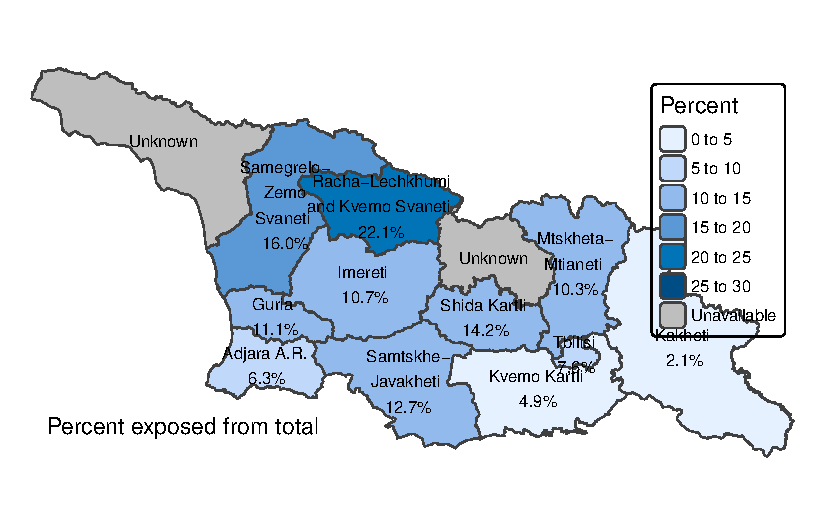
\includegraphics{vulnerability_files/figure-pdf/fig-exposed-total-1.pdf}

}

\caption{\label{fig-exposed-total}Percent exposed from total}

\end{figure}%

\subsection{Exposed and poor}\label{exposed-and-poor}

\begin{Shaded}
\begin{Highlighting}[]
\NormalTok{map\_object }\OtherTok{\textless{}{-}}
\FunctionTok{tm\_shape}\NormalTok{(exposed\_and\_poor\_map)}\SpecialCharTok{+}
  \FunctionTok{tm\_polygons}\NormalTok{(}\StringTok{"Pct. Below PL from exposed"}\NormalTok{,}
              \AttributeTok{title=}\StringTok{"Percent"}\NormalTok{, }
              \AttributeTok{legend.show =} \ConstantTok{TRUE}\NormalTok{,}
              \AttributeTok{style =} \StringTok{"fixed"}\NormalTok{,}
              \AttributeTok{scale =} \DecValTok{5}\NormalTok{,}
              \AttributeTok{breaks =} \FunctionTok{c}\NormalTok{(}\DecValTok{0}\NormalTok{, }\DecValTok{5}\NormalTok{, }\DecValTok{10}\NormalTok{, }\DecValTok{15}\NormalTok{, }\DecValTok{20}\NormalTok{, }\DecValTok{25}\NormalTok{, }\DecValTok{30}\NormalTok{),}
              \AttributeTok{textNA =} \StringTok{"Unavailable"}\NormalTok{,}
              \AttributeTok{colorNA =} \StringTok{"grey"}
\NormalTok{              ) }\SpecialCharTok{+}
  \FunctionTok{tm\_text}\NormalTok{(}\FunctionTok{c}\NormalTok{(}\StringTok{"pct\_exposed\_poor\_label"}\NormalTok{), }\AttributeTok{size =}\NormalTok{ .}\DecValTok{7}\NormalTok{, }\AttributeTok{col =} \StringTok{"black"}\NormalTok{)}\SpecialCharTok{+}
  \FunctionTok{tm\_layout}\NormalTok{(}
    \CommentTok{\#legend.outside = TRUE,}
    \AttributeTok{legend.position =} \FunctionTok{c}\NormalTok{(}\StringTok{"right"}\NormalTok{, }\StringTok{"top"}\NormalTok{),}
    \CommentTok{\#title.snap.to.legend = FALSE,}
    \AttributeTok{title =} 
      \StringTok{"Percent below poverty line}\SpecialCharTok{\textbackslash{}n}\StringTok{from those exposed"}\NormalTok{,}
    \AttributeTok{frame =} \ConstantTok{FALSE}\NormalTok{,}
\CommentTok{\#            outer.margins=c(.10,.10, .10, .10), }
            \AttributeTok{title.position =} \FunctionTok{c}\NormalTok{(}\StringTok{\textquotesingle{}left\textquotesingle{}}\NormalTok{, }\StringTok{\textquotesingle{}bottom\textquotesingle{}}\NormalTok{),}
            \AttributeTok{title.size =} \FloatTok{0.9}\NormalTok{)}

\FunctionTok{tmap\_save}\NormalTok{(}
\NormalTok{  map\_object,}
  \StringTok{"data/outputs/vulnerability\_img/pct\_flood\_poor\_fm\_exposed.svg"}\NormalTok{,}
  \AttributeTok{width =} \DecValTok{8}\NormalTok{,}
  \AttributeTok{height =} \DecValTok{5}\NormalTok{,}
  \AttributeTok{units =} \StringTok{"in"}
\NormalTok{)}
\NormalTok{map\_object}
\end{Highlighting}
\end{Shaded}

\begin{figure}[H]

\centering{

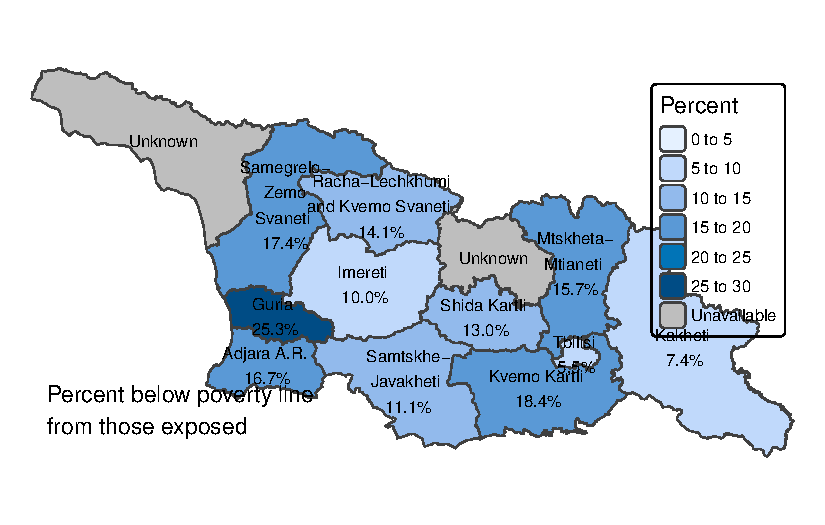
\includegraphics{vulnerability_files/figure-pdf/fig-exposed-and-poor-1.pdf}

}

\caption{\label{fig-exposed-and-poor}Percent below poverty line from
those exposed}

\end{figure}%

\subsection{At risk by dimension}\label{at-risk-by-dimension}

\begin{Shaded}
\begin{Highlighting}[]
\NormalTok{at\_risk\_map }\OtherTok{\textless{}{-}}\NormalTok{ adm1 }\SpecialCharTok{|\textgreater{}} 
  \FunctionTok{left\_join}\NormalTok{(}
\NormalTok{    at\_risk,}
    \FunctionTok{join\_by}\NormalTok{(region }\SpecialCharTok{==}\NormalTok{ Regions)}
\NormalTok{  ) }\SpecialCharTok{|\textgreater{}} 
  \FunctionTok{mutate}\NormalTok{(}
    \AttributeTok{region =} \FunctionTok{case\_when}\NormalTok{(}
\NormalTok{      region }\SpecialCharTok{==} \StringTok{"Racha{-}Lechkhumi and Kvemo Svaneti"} \SpecialCharTok{\textasciitilde{}}
      \StringTok{"Racha{-}Lechkhumi}\SpecialCharTok{\textbackslash{}n}\StringTok{and Kvemo Svaneti"}\NormalTok{,}
\NormalTok{      region }\SpecialCharTok{==} \StringTok{"Samegrelo{-}Zemo Svaneti"} \SpecialCharTok{\textasciitilde{}}
      \StringTok{"Samegrelo{-}}\SpecialCharTok{\textbackslash{}n}\StringTok{Zemo}\SpecialCharTok{\textbackslash{}n}\StringTok{Svaneti"}\NormalTok{,}
\NormalTok{      region }\SpecialCharTok{==} \StringTok{"Mtskheta{-}Mtianeti"} \SpecialCharTok{\textasciitilde{}}
      \StringTok{"Mtskheta{-}}\SpecialCharTok{\textbackslash{}n}\StringTok{Mtianeti"}\NormalTok{,}
\NormalTok{      region }\SpecialCharTok{==} \StringTok{"Samtskhe{-}Javakheti"} \SpecialCharTok{\textasciitilde{}}
      \StringTok{"Samtskhe{-}}\SpecialCharTok{\textbackslash{}n}\StringTok{Javakheti"}\NormalTok{,}
      \AttributeTok{.default =}\NormalTok{ region}
\NormalTok{    ),}
    \AttributeTok{pct\_income =}\NormalTok{ Income }\SpecialCharTok{/} \StringTok{\textasciigrave{}}\AttributeTok{Total Exposed}\StringTok{\textasciigrave{}} \SpecialCharTok{*} \DecValTok{100}\NormalTok{,}
    \AttributeTok{pct\_education =}\NormalTok{ Education  }\SpecialCharTok{/} \StringTok{\textasciigrave{}}\AttributeTok{Total Exposed}\StringTok{\textasciigrave{}} \SpecialCharTok{*} \DecValTok{100}\NormalTok{,}
    \AttributeTok{pct\_water =}\NormalTok{ Water }\SpecialCharTok{/} \StringTok{\textasciigrave{}}\AttributeTok{Total Exposed}\StringTok{\textasciigrave{}} \SpecialCharTok{*} \DecValTok{100}\NormalTok{,}
    \AttributeTok{pct\_sanitation =}\NormalTok{ Sanitation  }\SpecialCharTok{/} \StringTok{\textasciigrave{}}\AttributeTok{Total Exposed}\StringTok{\textasciigrave{}} \SpecialCharTok{*} \DecValTok{100}\NormalTok{,}
    \AttributeTok{pct\_buildings =}\NormalTok{ Buildings }\SpecialCharTok{/} \StringTok{\textasciigrave{}}\AttributeTok{Total Exposed}\StringTok{\textasciigrave{}} \SpecialCharTok{*} \DecValTok{100}\NormalTok{,}
    \AttributeTok{pct\_ssp =} \StringTok{\textasciigrave{}}\AttributeTok{Social Protection}\StringTok{\textasciigrave{}} \SpecialCharTok{/} \StringTok{\textasciigrave{}}\AttributeTok{Total Exposed}\StringTok{\textasciigrave{}} \SpecialCharTok{*} \DecValTok{100}\NormalTok{,}
    \AttributeTok{pct\_financial =} \StringTok{\textasciigrave{}}\AttributeTok{Financial inclusion}\StringTok{\textasciigrave{}} \SpecialCharTok{/} \StringTok{\textasciigrave{}}\AttributeTok{Total Exposed}\StringTok{\textasciigrave{}} \SpecialCharTok{*} \DecValTok{100}\NormalTok{,}
    \AttributeTok{pct\_income\_label =} \FunctionTok{if\_else}\NormalTok{(}
      \FunctionTok{is.na}\NormalTok{(Income), }
      \ConstantTok{NA}\NormalTok{, }
      \FunctionTok{paste}\NormalTok{(}
\NormalTok{        region,}
        \FunctionTok{sprintf}\NormalTok{(}\StringTok{"}\SpecialCharTok{\textbackslash{}n}\StringTok{\%.1f\%\%"}\NormalTok{, pct\_income)}
\NormalTok{      ) }
\NormalTok{    ),}
    \AttributeTok{pct\_education\_label =} \FunctionTok{if\_else}\NormalTok{(}
      \FunctionTok{is.na}\NormalTok{(Education), }
      \ConstantTok{NA}\NormalTok{, }
      \FunctionTok{paste}\NormalTok{(}
\NormalTok{        region,}
        \FunctionTok{sprintf}\NormalTok{(}\StringTok{"}\SpecialCharTok{\textbackslash{}n}\StringTok{\%.1f\%\%"}\NormalTok{, pct\_education)}
\NormalTok{      ) }
\NormalTok{    ),}
    \AttributeTok{pct\_water\_label =} \FunctionTok{if\_else}\NormalTok{(}
      \FunctionTok{is.na}\NormalTok{(Water), }
      \ConstantTok{NA}\NormalTok{, }
      \FunctionTok{paste}\NormalTok{(}
\NormalTok{        region,}
        \FunctionTok{sprintf}\NormalTok{(}\StringTok{"}\SpecialCharTok{\textbackslash{}n}\StringTok{\%.1f\%\%"}\NormalTok{, pct\_water)}
\NormalTok{      ) }
\NormalTok{    ),}
    \AttributeTok{pct\_sanitation\_label =} \FunctionTok{if\_else}\NormalTok{(}
      \FunctionTok{is.na}\NormalTok{(Sanitation), }
      \ConstantTok{NA}\NormalTok{, }
      \FunctionTok{paste}\NormalTok{(}
\NormalTok{        region,}
        \FunctionTok{sprintf}\NormalTok{(}\StringTok{"}\SpecialCharTok{\textbackslash{}n}\StringTok{\%.1f\%\%"}\NormalTok{, pct\_sanitation)}
\NormalTok{      ) }
\NormalTok{    ),}
    \AttributeTok{pct\_buildings\_label =} \FunctionTok{if\_else}\NormalTok{(}
      \FunctionTok{is.na}\NormalTok{(Buildings), }
      \ConstantTok{NA}\NormalTok{, }
      \FunctionTok{paste}\NormalTok{(}
\NormalTok{        region,}
        \FunctionTok{sprintf}\NormalTok{(}\StringTok{"}\SpecialCharTok{\textbackslash{}n}\StringTok{\%.1f\%\%"}\NormalTok{, pct\_buildings)}
\NormalTok{      ) }
\NormalTok{    ),}
    \AttributeTok{pct\_ssp\_label =} \FunctionTok{if\_else}\NormalTok{(}
      \FunctionTok{is.na}\NormalTok{(}\StringTok{\textasciigrave{}}\AttributeTok{Social Protection}\StringTok{\textasciigrave{}}\NormalTok{), }
      \ConstantTok{NA}\NormalTok{, }
      \FunctionTok{paste}\NormalTok{(}
\NormalTok{        region,}
        \FunctionTok{sprintf}\NormalTok{(}\StringTok{"}\SpecialCharTok{\textbackslash{}n}\StringTok{\%.1f\%\%"}\NormalTok{, pct\_ssp)}
\NormalTok{      ) }
\NormalTok{    ),}
    \AttributeTok{pct\_financial\_label =} \FunctionTok{if\_else}\NormalTok{(}
      \FunctionTok{is.na}\NormalTok{(}\StringTok{\textasciigrave{}}\AttributeTok{Financial inclusion}\StringTok{\textasciigrave{}}\NormalTok{), }
      \ConstantTok{NA}\NormalTok{, }
      \FunctionTok{paste}\NormalTok{(}
\NormalTok{        region,}
        \FunctionTok{sprintf}\NormalTok{(}\StringTok{"}\SpecialCharTok{\textbackslash{}n}\StringTok{\%.1f\%\%"}\NormalTok{, pct\_financial)}
\NormalTok{      ) }
\NormalTok{    )}
\NormalTok{  )}
\end{Highlighting}
\end{Shaded}

\subsubsection{Income}\label{income-1}

\begin{Shaded}
\begin{Highlighting}[]
\NormalTok{map\_object }\OtherTok{\textless{}{-}}
\FunctionTok{tm\_shape}\NormalTok{(at\_risk\_map)}\SpecialCharTok{+}
  \FunctionTok{tm\_polygons}\NormalTok{(}\StringTok{"pct\_income"}\NormalTok{,}
              \AttributeTok{title=}\StringTok{"Percent"}\NormalTok{, }
              \AttributeTok{legend.show =} \ConstantTok{TRUE}\NormalTok{,}
              \AttributeTok{style =} \StringTok{"fixed"}\NormalTok{,}
              \AttributeTok{scale =} \DecValTok{10}\NormalTok{,}
              \AttributeTok{breaks =} \FunctionTok{c}\NormalTok{(}\DecValTok{0}\NormalTok{, }\DecValTok{10}\NormalTok{, }\DecValTok{20}\NormalTok{, }\DecValTok{30}\NormalTok{, }\DecValTok{40}\NormalTok{, }\DecValTok{50}\NormalTok{, }\DecValTok{60}\NormalTok{),}
              \AttributeTok{palette =} \StringTok{"Blues"}\NormalTok{,}
              \AttributeTok{textNA =} \StringTok{"Unavailable"}\NormalTok{,}
              \AttributeTok{colorNA =} \StringTok{"grey"}
\NormalTok{              ) }\SpecialCharTok{+}
  \FunctionTok{tm\_text}\NormalTok{(}\FunctionTok{c}\NormalTok{(}\StringTok{"pct\_income\_label"}\NormalTok{), }\AttributeTok{size =}\NormalTok{ .}\DecValTok{7}\NormalTok{, }\AttributeTok{col =} \StringTok{"black"}\NormalTok{)}\SpecialCharTok{+}
  \FunctionTok{tm\_layout}\NormalTok{(}
    \CommentTok{\#legend.outside = TRUE,}
    \AttributeTok{legend.position =} \FunctionTok{c}\NormalTok{(}\StringTok{"right"}\NormalTok{, }\StringTok{"top"}\NormalTok{),}
    \CommentTok{\#title.snap.to.legend = FALSE,}
    \AttributeTok{title =} 
      \StringTok{"Percent income dimension}\SpecialCharTok{\textbackslash{}n}\StringTok{from those exposed"}\NormalTok{,}
    \AttributeTok{frame =} \ConstantTok{FALSE}\NormalTok{,}
\CommentTok{\#            outer.margins=c(.10,.10, .10, .10), }
            \AttributeTok{title.position =} \FunctionTok{c}\NormalTok{(}\StringTok{\textquotesingle{}left\textquotesingle{}}\NormalTok{, }\StringTok{\textquotesingle{}bottom\textquotesingle{}}\NormalTok{),}
            \AttributeTok{title.size =} \FloatTok{0.9}\NormalTok{)}

\FunctionTok{tmap\_save}\NormalTok{(}
\NormalTok{  map\_object,}
  \StringTok{"data/outputs/vulnerability\_img/pct\_flood\_income.svg"}\NormalTok{,}
  \AttributeTok{width =} \DecValTok{8}\NormalTok{,}
  \AttributeTok{height =} \DecValTok{5}\NormalTok{,}
  \AttributeTok{units =} \StringTok{"in"}
\NormalTok{)}
\NormalTok{map\_object}
\end{Highlighting}
\end{Shaded}

\begin{figure}[H]

\centering{

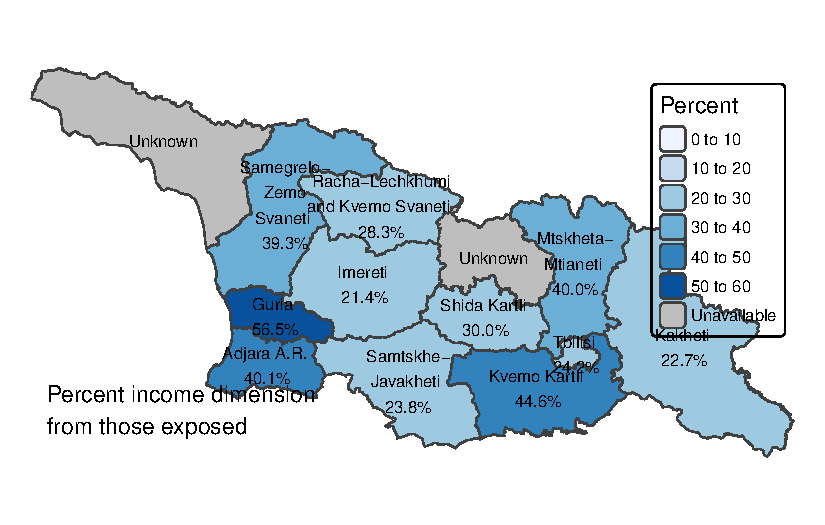
\includegraphics{vulnerability_files/figure-pdf/fig-income-1.pdf}

}

\caption{\label{fig-income}Percent with income dimension from those
exposed}

\end{figure}%

\subsubsection{Education}\label{education-1}

\begin{Shaded}
\begin{Highlighting}[]
\NormalTok{map\_object }\OtherTok{\textless{}{-}}
\FunctionTok{tm\_shape}\NormalTok{(at\_risk\_map)}\SpecialCharTok{+}
  \FunctionTok{tm\_polygons}\NormalTok{(}\StringTok{"pct\_education"}\NormalTok{,}
              \AttributeTok{title=}\StringTok{"Percent"}\NormalTok{, }
              \AttributeTok{legend.show =} \ConstantTok{TRUE}\NormalTok{,}
              \AttributeTok{style =} \StringTok{"fixed"}\NormalTok{,}
              \AttributeTok{scale =} \DecValTok{10}\NormalTok{,}
              \AttributeTok{breaks =} \FunctionTok{c}\NormalTok{(}\DecValTok{0}\NormalTok{, }\DecValTok{10}\NormalTok{, }\DecValTok{20}\NormalTok{, }\DecValTok{30}\NormalTok{, }\DecValTok{40}\NormalTok{, }\DecValTok{50}\NormalTok{, }\DecValTok{60}\NormalTok{),}
              \AttributeTok{palette =} \StringTok{"Blues"}\NormalTok{,}
              \AttributeTok{textNA =} \StringTok{"Unavailable"}\NormalTok{,}
              \AttributeTok{colorNA =} \StringTok{"grey"}
\NormalTok{              ) }\SpecialCharTok{+}
  \FunctionTok{tm\_text}\NormalTok{(}\FunctionTok{c}\NormalTok{(}\StringTok{"pct\_education\_label"}\NormalTok{), }\AttributeTok{size =}\NormalTok{ .}\DecValTok{7}\NormalTok{, }\AttributeTok{col =} \StringTok{"black"}\NormalTok{)}\SpecialCharTok{+}
  \FunctionTok{tm\_layout}\NormalTok{(}
    \CommentTok{\#legend.outside = TRUE,}
    \AttributeTok{legend.position =} \FunctionTok{c}\NormalTok{(}\StringTok{"right"}\NormalTok{, }\StringTok{"top"}\NormalTok{),}
    \CommentTok{\#title.snap.to.legend = FALSE,}
    \AttributeTok{title =} 
      \StringTok{"Percent education dimension}\SpecialCharTok{\textbackslash{}n}\StringTok{from those exposed"}\NormalTok{,}
    \AttributeTok{frame =} \ConstantTok{FALSE}\NormalTok{,}
\CommentTok{\#            outer.margins=c(.10,.10, .10, .10), }
            \AttributeTok{title.position =} \FunctionTok{c}\NormalTok{(}\StringTok{\textquotesingle{}left\textquotesingle{}}\NormalTok{, }\StringTok{\textquotesingle{}bottom\textquotesingle{}}\NormalTok{),}
            \AttributeTok{title.size =} \FloatTok{0.9}\NormalTok{)}

\FunctionTok{tmap\_save}\NormalTok{(}
\NormalTok{  map\_object,}
  \StringTok{"data/outputs/vulnerability\_img/pct\_flood\_education.svg"}\NormalTok{,}
  \AttributeTok{width =} \DecValTok{8}\NormalTok{,}
  \AttributeTok{height =} \DecValTok{5}\NormalTok{,}
  \AttributeTok{units =} \StringTok{"in"}
\NormalTok{)}
\NormalTok{map\_object}
\end{Highlighting}
\end{Shaded}

\begin{figure}[H]

\centering{

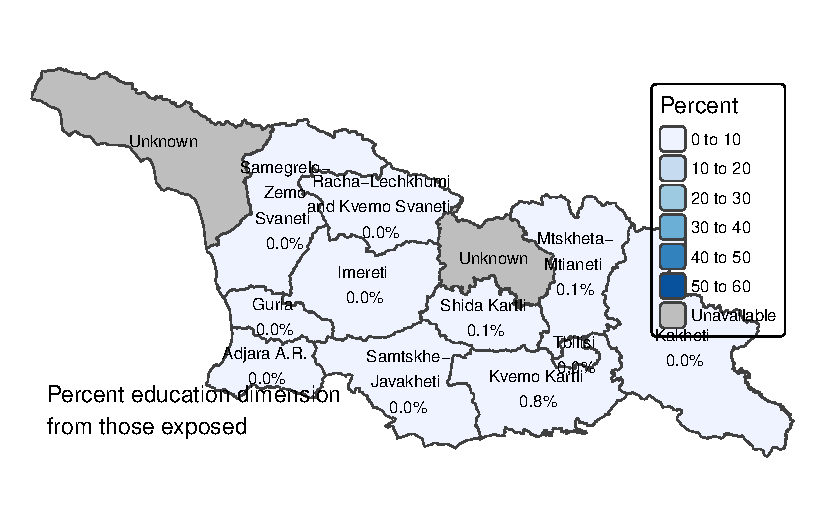
\includegraphics{vulnerability_files/figure-pdf/fig-education-1.pdf}

}

\caption{\label{fig-education}Percent with education dimension from
those exposed}

\end{figure}%

\subsubsection{Water}\label{water}

\begin{Shaded}
\begin{Highlighting}[]
\NormalTok{map\_object }\OtherTok{\textless{}{-}}
\FunctionTok{tm\_shape}\NormalTok{(at\_risk\_map)}\SpecialCharTok{+}
  \FunctionTok{tm\_polygons}\NormalTok{(}\StringTok{"pct\_water"}\NormalTok{,}
              \AttributeTok{title=}\StringTok{"Percent"}\NormalTok{, }
              \AttributeTok{legend.show =} \ConstantTok{TRUE}\NormalTok{,}
              \AttributeTok{style =} \StringTok{"fixed"}\NormalTok{,}
              \AttributeTok{scale =} \DecValTok{10}\NormalTok{,}
              \AttributeTok{breaks =} \FunctionTok{c}\NormalTok{(}\DecValTok{0}\NormalTok{, }\DecValTok{10}\NormalTok{, }\DecValTok{20}\NormalTok{, }\DecValTok{30}\NormalTok{, }\DecValTok{40}\NormalTok{, }\DecValTok{50}\NormalTok{, }\DecValTok{60}\NormalTok{),}
              \AttributeTok{palette =} \StringTok{"Blues"}\NormalTok{,}
              \AttributeTok{textNA =} \StringTok{"Unavailable"}\NormalTok{,}
              \AttributeTok{colorNA =} \StringTok{"grey"}
\NormalTok{              ) }\SpecialCharTok{+}
  \FunctionTok{tm\_text}\NormalTok{(}\FunctionTok{c}\NormalTok{(}\StringTok{"pct\_water\_label"}\NormalTok{), }\AttributeTok{size =}\NormalTok{ .}\DecValTok{7}\NormalTok{, }\AttributeTok{col =} \StringTok{"black"}\NormalTok{)}\SpecialCharTok{+}
  \FunctionTok{tm\_layout}\NormalTok{(}
    \CommentTok{\#legend.outside = TRUE,}
    \AttributeTok{legend.position =} \FunctionTok{c}\NormalTok{(}\StringTok{"right"}\NormalTok{, }\StringTok{"top"}\NormalTok{),}
    \CommentTok{\#title.snap.to.legend = FALSE,}
    \AttributeTok{title =} 
      \StringTok{"Percent water dimension}\SpecialCharTok{\textbackslash{}n}\StringTok{from those exposed"}\NormalTok{,}
    \AttributeTok{frame =} \ConstantTok{FALSE}\NormalTok{,}
\CommentTok{\#            outer.margins=c(.10,.10, .10, .10), }
            \AttributeTok{title.position =} \FunctionTok{c}\NormalTok{(}\StringTok{\textquotesingle{}left\textquotesingle{}}\NormalTok{, }\StringTok{\textquotesingle{}bottom\textquotesingle{}}\NormalTok{),}
            \AttributeTok{title.size =} \FloatTok{0.9}\NormalTok{)}

\FunctionTok{tmap\_save}\NormalTok{(}
\NormalTok{  map\_object,}
  \StringTok{"data/outputs/vulnerability\_img/pct\_flood\_water.svg"}\NormalTok{,}
  \AttributeTok{width =} \DecValTok{8}\NormalTok{,}
  \AttributeTok{height =} \DecValTok{5}\NormalTok{,}
  \AttributeTok{units =} \StringTok{"in"}
\NormalTok{)}
\NormalTok{map\_object}
\end{Highlighting}
\end{Shaded}

\begin{figure}[H]

\centering{

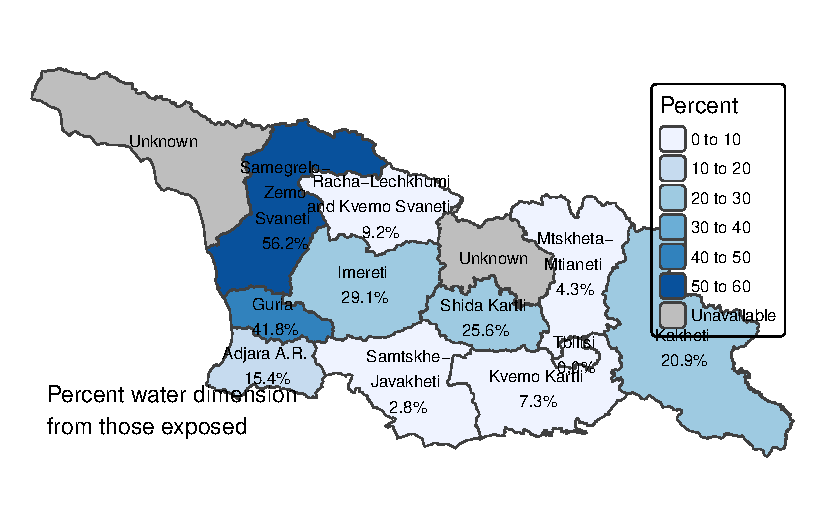
\includegraphics{vulnerability_files/figure-pdf/fig-water-1.pdf}

}

\caption{\label{fig-water}Percent with water dimension from those
exposed}

\end{figure}%

\subsubsection{Sanitation}\label{sanitation}

\begin{Shaded}
\begin{Highlighting}[]
\NormalTok{map\_object }\OtherTok{\textless{}{-}}
\FunctionTok{tm\_shape}\NormalTok{(at\_risk\_map)}\SpecialCharTok{+}
  \FunctionTok{tm\_polygons}\NormalTok{(}\StringTok{"pct\_sanitation"}\NormalTok{,}
              \AttributeTok{title=}\StringTok{"Percent"}\NormalTok{, }
              \AttributeTok{legend.show =} \ConstantTok{TRUE}\NormalTok{,}
              \AttributeTok{style =} \StringTok{"fixed"}\NormalTok{,}
              \AttributeTok{scale =} \DecValTok{20}\NormalTok{,}
              \AttributeTok{breaks =} \FunctionTok{c}\NormalTok{(}\DecValTok{0}\NormalTok{, }\DecValTok{20}\NormalTok{, }\DecValTok{40}\NormalTok{, }\DecValTok{60}\NormalTok{, }\DecValTok{80}\NormalTok{, }\DecValTok{100}\NormalTok{),}
              \AttributeTok{palette =} \StringTok{"Blues"}\NormalTok{,}
              \AttributeTok{textNA =} \StringTok{"Unavailable"}\NormalTok{,}
              \AttributeTok{colorNA =} \StringTok{"grey"}
\NormalTok{              ) }\SpecialCharTok{+}
  \FunctionTok{tm\_text}\NormalTok{(}\FunctionTok{c}\NormalTok{(}\StringTok{"pct\_sanitation\_label"}\NormalTok{), }\AttributeTok{size =}\NormalTok{ .}\DecValTok{7}\NormalTok{, }\AttributeTok{col =} \StringTok{"black"}\NormalTok{)}\SpecialCharTok{+}
  \FunctionTok{tm\_layout}\NormalTok{(}
    \CommentTok{\#legend.outside = TRUE,}
    \AttributeTok{legend.position =} \FunctionTok{c}\NormalTok{(}\StringTok{"right"}\NormalTok{, }\StringTok{"top"}\NormalTok{),}
    \CommentTok{\#title.snap.to.legend = FALSE,}
    \AttributeTok{title =} 
      \StringTok{"Percent sanitation dimension}\SpecialCharTok{\textbackslash{}n}\StringTok{from those exposed"}\NormalTok{,}
    \AttributeTok{frame =} \ConstantTok{FALSE}\NormalTok{,}
\CommentTok{\#            outer.margins=c(.10,.10, .10, .10), }
            \AttributeTok{title.position =} \FunctionTok{c}\NormalTok{(}\StringTok{\textquotesingle{}left\textquotesingle{}}\NormalTok{, }\StringTok{\textquotesingle{}bottom\textquotesingle{}}\NormalTok{),}
            \AttributeTok{title.size =} \FloatTok{0.9}\NormalTok{)}

\FunctionTok{tmap\_save}\NormalTok{(}
\NormalTok{  map\_object,}
  \StringTok{"data/outputs/vulnerability\_img/pct\_flood\_sanitation.svg"}\NormalTok{,}
  \AttributeTok{width =} \DecValTok{8}\NormalTok{,}
  \AttributeTok{height =} \DecValTok{5}\NormalTok{,}
  \AttributeTok{units =} \StringTok{"in"}
\NormalTok{)}
\NormalTok{map\_object}
\end{Highlighting}
\end{Shaded}

\begin{figure}[H]

\centering{

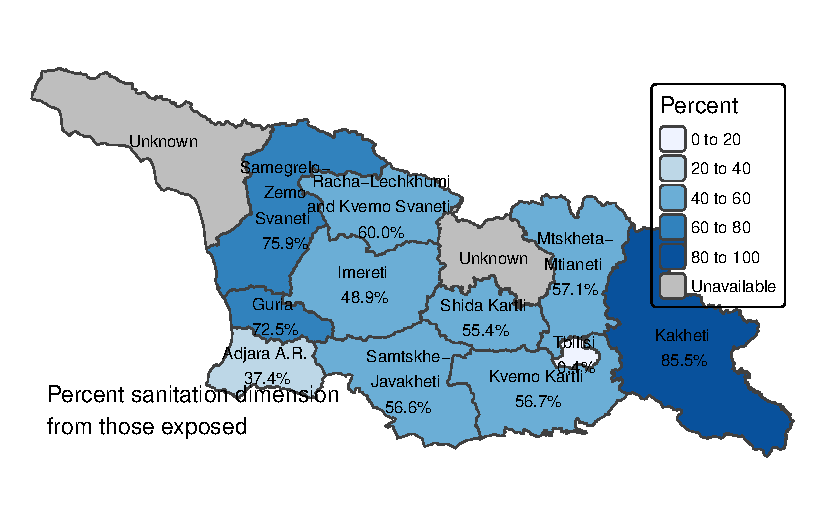
\includegraphics{vulnerability_files/figure-pdf/fig-sanitation-1.pdf}

}

\caption{\label{fig-sanitation}Percent with sanitation dimension from
those exposed}

\end{figure}%

\subsubsection{Building materials}\label{building-materials-1}

\begin{Shaded}
\begin{Highlighting}[]
\NormalTok{map\_object }\OtherTok{\textless{}{-}}
\FunctionTok{tm\_shape}\NormalTok{(at\_risk\_map)}\SpecialCharTok{+}
  \FunctionTok{tm\_polygons}\NormalTok{(}\StringTok{"pct\_buildings"}\NormalTok{,}
              \AttributeTok{title=}\StringTok{"Percent"}\NormalTok{, }
              \AttributeTok{legend.show =} \ConstantTok{TRUE}\NormalTok{,}
              \AttributeTok{style =} \StringTok{"fixed"}\NormalTok{,}
              \AttributeTok{scale =} \DecValTok{10}\NormalTok{,}
              \AttributeTok{breaks =} \FunctionTok{c}\NormalTok{(}\DecValTok{0}\NormalTok{, }\DecValTok{10}\NormalTok{, }\DecValTok{20}\NormalTok{, }\DecValTok{30}\NormalTok{, }\DecValTok{40}\NormalTok{, }\DecValTok{50}\NormalTok{, }\DecValTok{60}\NormalTok{),}
              \AttributeTok{palette =} \StringTok{"Blues"}\NormalTok{,}
              \AttributeTok{textNA =} \StringTok{"Unavailable"}\NormalTok{,}
              \AttributeTok{colorNA =} \StringTok{"grey"}
\NormalTok{              ) }\SpecialCharTok{+}
  \FunctionTok{tm\_text}\NormalTok{(}\FunctionTok{c}\NormalTok{(}\StringTok{"pct\_buildings\_label"}\NormalTok{), }\AttributeTok{size =}\NormalTok{ .}\DecValTok{7}\NormalTok{, }\AttributeTok{col =} \StringTok{"black"}\NormalTok{)}\SpecialCharTok{+}
  \FunctionTok{tm\_layout}\NormalTok{(}
    \CommentTok{\#legend.outside = TRUE,}
    \AttributeTok{legend.position =} \FunctionTok{c}\NormalTok{(}\StringTok{"right"}\NormalTok{, }\StringTok{"top"}\NormalTok{),}
    \CommentTok{\#title.snap.to.legend = FALSE,}
    \AttributeTok{title =} 
      \StringTok{"Percent building materials}\SpecialCharTok{\textbackslash{}n}\StringTok{dimension from those exposed"}\NormalTok{,}
    \AttributeTok{frame =} \ConstantTok{FALSE}\NormalTok{,}
\CommentTok{\#            outer.margins=c(.10,.10, .10, .10), }
            \AttributeTok{title.position =} \FunctionTok{c}\NormalTok{(}\StringTok{\textquotesingle{}left\textquotesingle{}}\NormalTok{, }\StringTok{\textquotesingle{}bottom\textquotesingle{}}\NormalTok{),}
            \AttributeTok{title.size =} \FloatTok{0.9}\NormalTok{)}

\FunctionTok{tmap\_save}\NormalTok{(}
\NormalTok{  map\_object,}
  \StringTok{"data/outputs/vulnerability\_img/pct\_flood\_buildings.svg"}\NormalTok{,}
  \AttributeTok{width =} \DecValTok{8}\NormalTok{,}
  \AttributeTok{height =} \DecValTok{5}\NormalTok{,}
  \AttributeTok{units =} \StringTok{"in"}
\NormalTok{)}
\NormalTok{map\_object}
\end{Highlighting}
\end{Shaded}

\begin{figure}[H]

\centering{

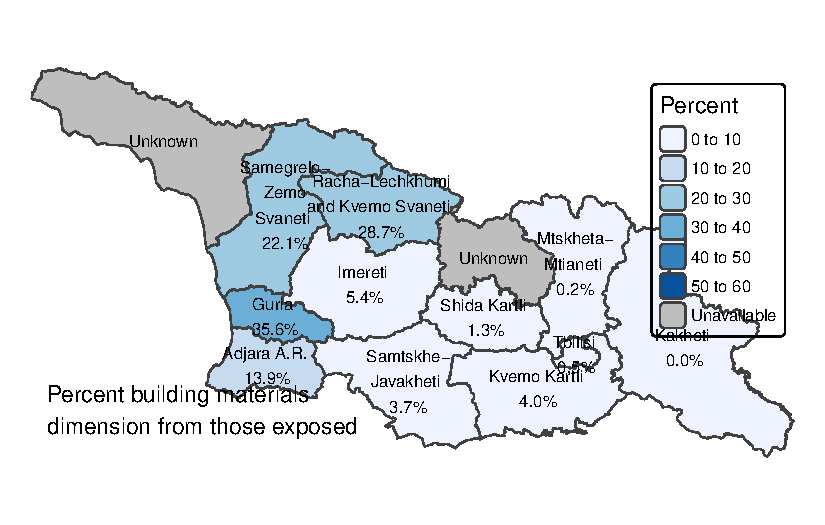
\includegraphics{vulnerability_files/figure-pdf/fig-buildings-1.pdf}

}

\caption{\label{fig-buildings}Percent with buildings dimension from
those exposed}

\end{figure}%

\subsubsection{Social protection}\label{social-protection-1}

\begin{Shaded}
\begin{Highlighting}[]
\NormalTok{map\_object }\OtherTok{\textless{}{-}}
\FunctionTok{tm\_shape}\NormalTok{(at\_risk\_map)}\SpecialCharTok{+}
  \FunctionTok{tm\_polygons}\NormalTok{(}\StringTok{"pct\_ssp"}\NormalTok{,}
              \AttributeTok{title=}\StringTok{"Percent"}\NormalTok{, }
              \AttributeTok{legend.show =} \ConstantTok{TRUE}\NormalTok{,}
              \AttributeTok{style =} \StringTok{"fixed"}\NormalTok{,}
              \AttributeTok{scale =} \DecValTok{10}\NormalTok{,}
              \AttributeTok{breaks =} \FunctionTok{c}\NormalTok{(}\DecValTok{50}\NormalTok{,}\DecValTok{60}\NormalTok{, }\DecValTok{70}\NormalTok{,}\DecValTok{80}\NormalTok{, }\DecValTok{90}\NormalTok{, }\DecValTok{100}\NormalTok{),}
              \AttributeTok{palette =} \StringTok{"Blues"}\NormalTok{,}
              \AttributeTok{textNA =} \StringTok{"Unavailable"}\NormalTok{,}
              \AttributeTok{colorNA =} \StringTok{"grey"}
\NormalTok{              ) }\SpecialCharTok{+}
  \FunctionTok{tm\_text}\NormalTok{(}\FunctionTok{c}\NormalTok{(}\StringTok{"pct\_ssp\_label"}\NormalTok{), }\AttributeTok{size =}\NormalTok{ .}\DecValTok{7}\NormalTok{, }\AttributeTok{col =} \StringTok{"black"}\NormalTok{)}\SpecialCharTok{+}
  \FunctionTok{tm\_layout}\NormalTok{(}
    \CommentTok{\#legend.outside = TRUE,}
    \AttributeTok{legend.position =} \FunctionTok{c}\NormalTok{(}\StringTok{"right"}\NormalTok{, }\StringTok{"top"}\NormalTok{),}
    \CommentTok{\#title.snap.to.legend = FALSE,}
    \AttributeTok{title =} 
      \StringTok{"Percent social protection}\SpecialCharTok{\textbackslash{}n}\StringTok{dimension from those exposed"}\NormalTok{,}
    \AttributeTok{frame =} \ConstantTok{FALSE}\NormalTok{,}
\CommentTok{\#            outer.margins=c(.10,.10, .10, .10), }
            \AttributeTok{title.position =} \FunctionTok{c}\NormalTok{(}\StringTok{\textquotesingle{}left\textquotesingle{}}\NormalTok{, }\StringTok{\textquotesingle{}bottom\textquotesingle{}}\NormalTok{),}
            \AttributeTok{title.size =} \FloatTok{0.9}\NormalTok{)}

\FunctionTok{tmap\_save}\NormalTok{(}
\NormalTok{  map\_object,}
  \StringTok{"data/outputs/vulnerability\_img/pct\_flood\_ssp.svg"}\NormalTok{,}
  \AttributeTok{width =} \DecValTok{8}\NormalTok{,}
  \AttributeTok{height =} \DecValTok{5}\NormalTok{,}
  \AttributeTok{units =} \StringTok{"in"}
\NormalTok{)}
\NormalTok{map\_object}
\end{Highlighting}
\end{Shaded}

\begin{figure}[H]

\centering{

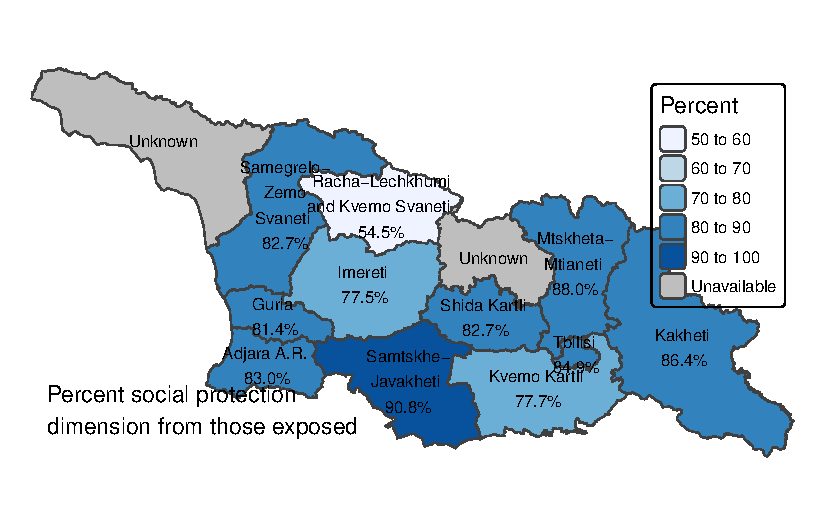
\includegraphics{vulnerability_files/figure-pdf/fig-ssp-1.pdf}

}

\caption{\label{fig-ssp}Percent with social dimension from those
exposed}

\end{figure}%

\subsubsection{Financial services}\label{financial-services-1}

\begin{Shaded}
\begin{Highlighting}[]
\NormalTok{map\_object }\OtherTok{\textless{}{-}}
\FunctionTok{tm\_shape}\NormalTok{(at\_risk\_map)}\SpecialCharTok{+}
  \FunctionTok{tm\_polygons}\NormalTok{(}\StringTok{"pct\_financial"}\NormalTok{,}
              \AttributeTok{title=}\StringTok{"Percent"}\NormalTok{, }
              \AttributeTok{legend.show =} \ConstantTok{TRUE}\NormalTok{,}
              \AttributeTok{style =} \StringTok{"fixed"}\NormalTok{,}
              \AttributeTok{scale =} \DecValTok{10}\NormalTok{,}
              \AttributeTok{breaks =} \FunctionTok{c}\NormalTok{(}\DecValTok{40}\NormalTok{, }\DecValTok{50}\NormalTok{,}\DecValTok{60}\NormalTok{, }\DecValTok{70}\NormalTok{,}\DecValTok{80}\NormalTok{, }\DecValTok{90}\NormalTok{, }\DecValTok{100}\NormalTok{),}
              \AttributeTok{palette =} \StringTok{"Blues"}\NormalTok{,}
              \AttributeTok{textNA =} \StringTok{"Unavailable"}\NormalTok{,}
              \AttributeTok{colorNA =} \StringTok{"grey"}
\NormalTok{              ) }\SpecialCharTok{+}
  \FunctionTok{tm\_text}\NormalTok{(}\FunctionTok{c}\NormalTok{(}\StringTok{"pct\_financial\_label"}\NormalTok{), }\AttributeTok{size =}\NormalTok{ .}\DecValTok{7}\NormalTok{, }\AttributeTok{col =} \StringTok{"black"}\NormalTok{)}\SpecialCharTok{+}
  \FunctionTok{tm\_layout}\NormalTok{(}
    \CommentTok{\#legend.outside = TRUE,}
    \AttributeTok{legend.position =} \FunctionTok{c}\NormalTok{(}\StringTok{"right"}\NormalTok{, }\StringTok{"top"}\NormalTok{),}
    \CommentTok{\#title.snap.to.legend = FALSE,}
    \AttributeTok{title =} 
      \StringTok{"Percent financial dimension}\SpecialCharTok{\textbackslash{}n}\StringTok{from those exposed"}\NormalTok{,}
    \AttributeTok{frame =} \ConstantTok{FALSE}\NormalTok{,}
\CommentTok{\#            outer.margins=c(.10,.10, .10, .10), }
            \AttributeTok{title.position =} \FunctionTok{c}\NormalTok{(}\StringTok{\textquotesingle{}left\textquotesingle{}}\NormalTok{, }\StringTok{\textquotesingle{}bottom\textquotesingle{}}\NormalTok{),}
            \AttributeTok{title.size =} \FloatTok{0.9}\NormalTok{)}

\FunctionTok{tmap\_save}\NormalTok{(}
\NormalTok{  map\_object,}
  \StringTok{"data/outputs/vulnerability\_img/pct\_flood\_financial.svg"}\NormalTok{,}
  \AttributeTok{width =} \DecValTok{8}\NormalTok{,}
  \AttributeTok{height =} \DecValTok{5}\NormalTok{,}
  \AttributeTok{units =} \StringTok{"in"}
\NormalTok{)}
\NormalTok{map\_object}
\end{Highlighting}
\end{Shaded}

\begin{figure}[H]

\centering{

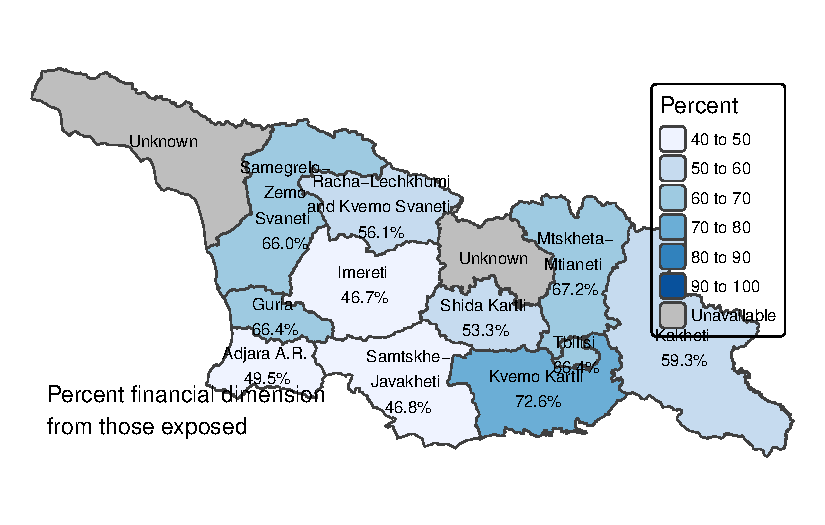
\includegraphics{vulnerability_files/figure-pdf/fig-financial-1.pdf}

}

\caption{\label{fig-financial}Percent with financial dimension from
those exposed}

\end{figure}%

\subsection{At risk by many
dimensions}\label{at-risk-by-many-dimensions}

Prepare map data

\begin{Shaded}
\begin{Highlighting}[]
\NormalTok{at\_risk\_dimensions\_map }\OtherTok{\textless{}{-}}\NormalTok{ adm1 }\SpecialCharTok{|\textgreater{}} 
  \FunctionTok{left\_join}\NormalTok{(}
\NormalTok{    at\_risk\_dimensions,}
    \FunctionTok{join\_by}\NormalTok{(region }\SpecialCharTok{==}\NormalTok{ Regions)}
\NormalTok{  ) }\SpecialCharTok{|\textgreater{}} 
  \FunctionTok{mutate}\NormalTok{(}
    \AttributeTok{region =} \FunctionTok{case\_when}\NormalTok{(}
\NormalTok{      region }\SpecialCharTok{==} \StringTok{"Racha{-}Lechkhumi and Kvemo Svaneti"} \SpecialCharTok{\textasciitilde{}}
      \StringTok{"Racha{-}Lechkhumi}\SpecialCharTok{\textbackslash{}n}\StringTok{and Kvemo Svaneti"}\NormalTok{,}
\NormalTok{      region }\SpecialCharTok{==} \StringTok{"Samegrelo{-}Zemo Svaneti"} \SpecialCharTok{\textasciitilde{}}
      \StringTok{"Samegrelo{-}}\SpecialCharTok{\textbackslash{}n}\StringTok{Zemo}\SpecialCharTok{\textbackslash{}n}\StringTok{Svaneti"}\NormalTok{,}
\NormalTok{      region }\SpecialCharTok{==} \StringTok{"Mtskheta{-}Mtianeti"} \SpecialCharTok{\textasciitilde{}}
      \StringTok{"Mtskheta{-}}\SpecialCharTok{\textbackslash{}n}\StringTok{Mtianeti"}\NormalTok{,}
\NormalTok{      region }\SpecialCharTok{==} \StringTok{"Samtskhe{-}Javakheti"} \SpecialCharTok{\textasciitilde{}}
      \StringTok{"Samtskhe{-}}\SpecialCharTok{\textbackslash{}n}\StringTok{Javakheti"}\NormalTok{,}
      \AttributeTok{.default =}\NormalTok{ region}
\NormalTok{    ),}
    \AttributeTok{up\_to\_2\_dims =} \FunctionTok{case\_when}\NormalTok{(}
      \FunctionTok{is.na}\NormalTok{(}\StringTok{\textasciigrave{}}\AttributeTok{1 dimension}\StringTok{\textasciigrave{}}\NormalTok{) }\SpecialCharTok{|} \FunctionTok{is.na}\NormalTok{(}\StringTok{\textasciigrave{}}\AttributeTok{2 dimensions}\StringTok{\textasciigrave{}}\NormalTok{) }\SpecialCharTok{\textasciitilde{}} \ConstantTok{NA}\NormalTok{,}
      \AttributeTok{.default =} \StringTok{\textasciigrave{}}\AttributeTok{1 dimension}\StringTok{\textasciigrave{}} \SpecialCharTok{+} \StringTok{\textasciigrave{}}\AttributeTok{2 dimensions}\StringTok{\textasciigrave{}}
\NormalTok{    ),}
    \AttributeTok{pct\_up\_to\_2\_dims =} \FunctionTok{if\_else}\NormalTok{(}
      \FunctionTok{is.na}\NormalTok{(}\StringTok{\textasciigrave{}}\AttributeTok{Total Exposed}\StringTok{\textasciigrave{}}\NormalTok{), }\StringTok{\textasciigrave{}}\AttributeTok{Total Exposed}\StringTok{\textasciigrave{}}\NormalTok{,}
\NormalTok{      up\_to\_2\_dims }\SpecialCharTok{/} \StringTok{\textasciigrave{}}\AttributeTok{Total Exposed}\StringTok{\textasciigrave{}} \SpecialCharTok{*} \DecValTok{100}
\NormalTok{    )}
\NormalTok{  ) }\SpecialCharTok{|\textgreater{}} 
  \FunctionTok{mutate}\NormalTok{(}
    \AttributeTok{pct\_up\_to\_2\_dims\_label =} \FunctionTok{if\_else}\NormalTok{(}
      \FunctionTok{is.na}\NormalTok{(pct\_up\_to\_2\_dims), }
      \ConstantTok{NA}\NormalTok{, }
      \FunctionTok{paste}\NormalTok{(}
\NormalTok{        region,}
        \FunctionTok{sprintf}\NormalTok{(}\StringTok{"}\SpecialCharTok{\textbackslash{}n}\StringTok{\%.1f\%\%"}\NormalTok{, pct\_up\_to\_2\_dims)}
\NormalTok{      ) }
\NormalTok{    )}
\NormalTok{  )}
\end{Highlighting}
\end{Shaded}

\begin{Shaded}
\begin{Highlighting}[]
\NormalTok{map\_object }\OtherTok{\textless{}{-}}
\FunctionTok{tm\_shape}\NormalTok{(at\_risk\_dimensions\_map)}\SpecialCharTok{+}
  \FunctionTok{tm\_polygons}\NormalTok{(}\StringTok{"pct\_up\_to\_2\_dims"}\NormalTok{,}
              \AttributeTok{title=}\StringTok{"Percent"}\NormalTok{, }
              \AttributeTok{legend.show =} \ConstantTok{TRUE}\NormalTok{,}
              \AttributeTok{style =} \StringTok{"fixed"}\NormalTok{,}
              \AttributeTok{scale =} \DecValTok{10}\NormalTok{,}
              \AttributeTok{breaks =} \FunctionTok{c}\NormalTok{(}\DecValTok{20}\NormalTok{,}\DecValTok{40}\NormalTok{, }\DecValTok{50}\NormalTok{,}\DecValTok{60}\NormalTok{, }\DecValTok{70}\NormalTok{,}\DecValTok{80}\NormalTok{, }\DecValTok{90}\NormalTok{,}\DecValTok{100}\NormalTok{),}
              \AttributeTok{palette =} \StringTok{"Purples"}\NormalTok{,}
              \AttributeTok{textNA =} \StringTok{"Unavailable"}\NormalTok{,}
              \AttributeTok{colorNA =} \StringTok{"grey"}
\NormalTok{              ) }\SpecialCharTok{+}
  \FunctionTok{tm\_text}\NormalTok{(}\FunctionTok{c}\NormalTok{(}\StringTok{"pct\_up\_to\_2\_dims\_label"}\NormalTok{), }\AttributeTok{size =}\NormalTok{ .}\DecValTok{7}\NormalTok{, }\AttributeTok{col =} \StringTok{"black"}\NormalTok{)}\SpecialCharTok{+}
  \FunctionTok{tm\_layout}\NormalTok{(}
    \CommentTok{\#legend.outside = TRUE,}
    \AttributeTok{legend.position =} \FunctionTok{c}\NormalTok{(}\StringTok{"right"}\NormalTok{, }\StringTok{"top"}\NormalTok{),}
    \CommentTok{\#title.snap.to.legend = FALSE,}
    \AttributeTok{title =} 
      \StringTok{"Percent with up to 2 dimensions}\SpecialCharTok{\textbackslash{}n}\StringTok{from those exposed"}\NormalTok{,}
    \AttributeTok{frame =} \ConstantTok{FALSE}\NormalTok{,}
\CommentTok{\#            outer.margins=c(.10,.10, .10, .10), }
            \AttributeTok{title.position =} \FunctionTok{c}\NormalTok{(}\StringTok{\textquotesingle{}left\textquotesingle{}}\NormalTok{, }\StringTok{\textquotesingle{}bottom\textquotesingle{}}\NormalTok{),}
            \AttributeTok{title.size =} \FloatTok{0.9}\NormalTok{)}

\FunctionTok{tmap\_save}\NormalTok{(}
\NormalTok{  map\_object,}
  \StringTok{"data/outputs/vulnerability\_img/pct\_flood\_up\_to\_2\_dimensions.svg"}\NormalTok{,}
  \AttributeTok{width =} \DecValTok{8}\NormalTok{,}
  \AttributeTok{height =} \DecValTok{5}\NormalTok{,}
  \AttributeTok{units =} \StringTok{"in"}
\NormalTok{)}
\NormalTok{map\_object}
\end{Highlighting}
\end{Shaded}

\begin{figure}[H]

\centering{

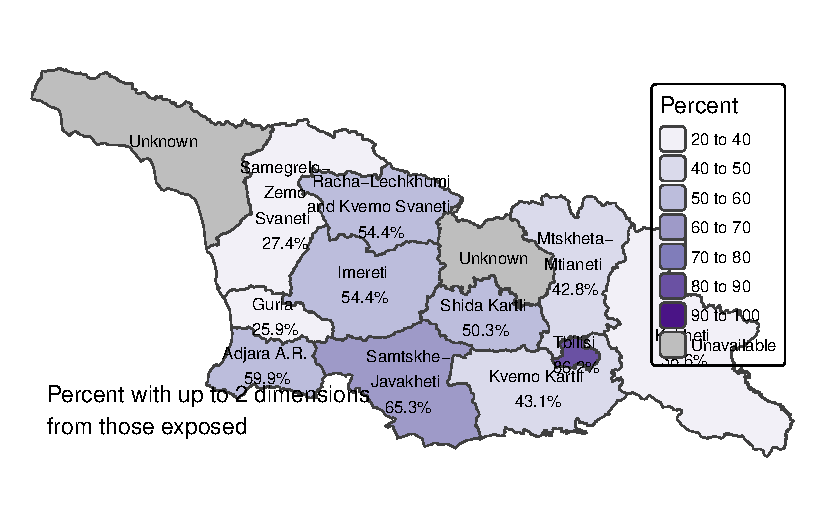
\includegraphics{vulnerability_files/figure-pdf/fig-up-to-2-dimensions-1.pdf}

}

\caption{\label{fig-up-to-2-dimensions}Percent with up to 2 dimensions
from those exposed}

\end{figure}%

\subsection{Spatially distributed
population}\label{spatially-distributed-population}

\begin{Shaded}
\begin{Highlighting}[]
\NormalTok{pop }\OtherTok{\textless{}{-}}\NormalTok{ raster}\SpecialCharTok{::}\FunctionTok{raster}\NormalTok{(}\StringTok{"data/gis/grided\_population\_2020.tif"}\NormalTok{)}

\NormalTok{map\_object }\OtherTok{\textless{}{-}}
\FunctionTok{tm\_shape}\NormalTok{(pop) }\SpecialCharTok{+}
  \FunctionTok{tm\_raster}\NormalTok{(}\StringTok{"grided\_population\_2020"}\NormalTok{, }
            \AttributeTok{style =} \StringTok{"fixed"}\NormalTok{, }
            \AttributeTok{breaks =} \FunctionTok{c}\NormalTok{(}\DecValTok{0}\NormalTok{, }\DecValTok{100}\NormalTok{, }\DecValTok{150}\NormalTok{, }\DecValTok{200}\NormalTok{, }\DecValTok{600}\NormalTok{, }\DecValTok{800}\NormalTok{, }\DecValTok{1000}\NormalTok{, }\DecValTok{10000}\NormalTok{),}
            \CommentTok{\# palette = "YlOrRd",}
            \AttributeTok{palette =} \StringTok{"BuPu"}\NormalTok{,}
            \AttributeTok{title =} \StringTok{"People per pixel"}\NormalTok{) }\SpecialCharTok{+}
  \FunctionTok{tm\_shape}\NormalTok{(adm1) }\SpecialCharTok{+}
  \FunctionTok{tm\_borders}\NormalTok{() }\SpecialCharTok{+}
  \FunctionTok{tm\_layout}\NormalTok{(}
    \AttributeTok{legend.position =} \FunctionTok{c}\NormalTok{(}\StringTok{"right"}\NormalTok{, }\StringTok{"top"}\NormalTok{),}
    \CommentTok{\#title.snap.to.legend = FALSE,}
    \AttributeTok{title =} 
      \StringTok{"Spatially distributed population layer"}\NormalTok{,}
    \AttributeTok{frame =} \ConstantTok{FALSE}\NormalTok{,}
\CommentTok{\#            outer.margins=c(.10,.10, .10, .10), }
            \AttributeTok{title.position =} \FunctionTok{c}\NormalTok{(}\StringTok{\textquotesingle{}left\textquotesingle{}}\NormalTok{, }\StringTok{\textquotesingle{}bottom\textquotesingle{}}\NormalTok{),}
            \AttributeTok{title.size =} \FloatTok{0.9}
\NormalTok{    )}

\FunctionTok{tmap\_save}\NormalTok{(}
\NormalTok{  map\_object,}
  \StringTok{"data/outputs/vulnerability\_img/gridded\_pop\_2020.svg"}\NormalTok{,}
  \AttributeTok{width =} \DecValTok{8}\NormalTok{,}
  \AttributeTok{height =} \DecValTok{5}\NormalTok{,}
  \AttributeTok{units =} \StringTok{"in"}
\NormalTok{)}
\NormalTok{map\_object}
\end{Highlighting}
\end{Shaded}

\begin{figure}[H]

\centering{

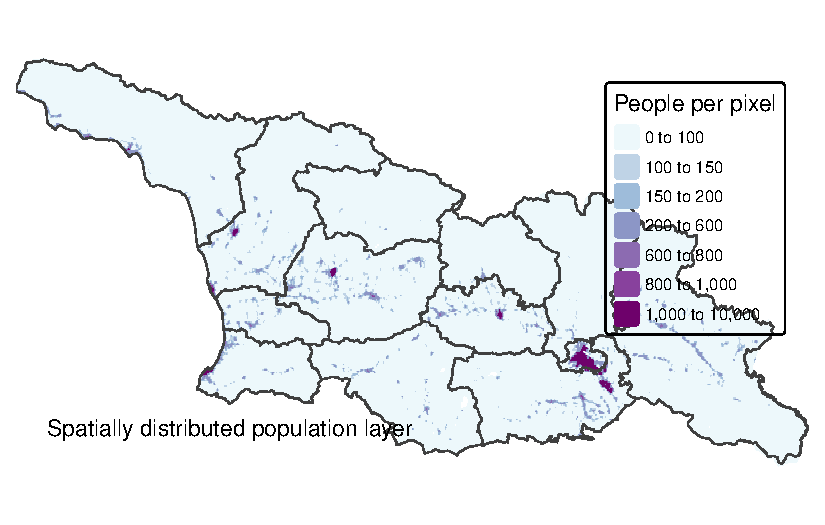
\includegraphics{vulnerability_files/figure-pdf/fig-gridded-population-1.pdf}

}

\caption{\label{fig-gridded-population}Spatially distributed population
layer}

\end{figure}%

\section{Exports to Excel}\label{exports-to-excel}

\begin{Shaded}
\begin{Highlighting}[]
\CommentTok{\# Define the file path}
\NormalTok{file\_path }\OtherTok{\textless{}{-}} \StringTok{"data/outputs/vulnerability.xlsx"}

\CommentTok{\# Check if the file exists}
\ControlFlowTok{if}\NormalTok{ (}\FunctionTok{file.exists}\NormalTok{(file\_path)) \{}
  \CommentTok{\# If the file exists, load the workbook}
\NormalTok{  wb }\OtherTok{\textless{}{-}} \FunctionTok{loadWorkbook}\NormalTok{(file\_path)}
\NormalTok{\} }\ControlFlowTok{else}\NormalTok{ \{}
  \CommentTok{\# If the file doesn\textquotesingle{}t exist, create a new workbook}
\NormalTok{  wb }\OtherTok{\textless{}{-}} \FunctionTok{createWorkbook}\NormalTok{()}
\NormalTok{\}}

\CommentTok{\# Print the sheet names in the workbook}
\NormalTok{sheet\_names }\OtherTok{\textless{}{-}} \FunctionTok{names}\NormalTok{(wb)}
\FunctionTok{print}\NormalTok{(sheet\_names)}
\end{Highlighting}
\end{Shaded}

\begin{verbatim}
[1] "Exposed and Poor"         "Exposed and Vulnerable"  
[3] "At Risk on Dimensions"    "exposure_pct"            
[5] "Traditionally Vulnerable"
\end{verbatim}

\begin{Shaded}
\begin{Highlighting}[]
\NormalTok{objects\_to\_add }\OtherTok{\textless{}{-}} \FunctionTok{c}\NormalTok{(}
  \StringTok{"exposed\_and\_poor"}\NormalTok{,}
  \StringTok{"at\_risk"}\NormalTok{,}
  \StringTok{"at\_risk\_dimensions"}\NormalTok{,}
  \StringTok{"exposure\_pct"}\NormalTok{,}
  \StringTok{"traditionally\_vulnerable\_area"}
\NormalTok{)}

\NormalTok{sheets\_to\_add }\OtherTok{\textless{}{-}} \FunctionTok{c}\NormalTok{(}
  \StringTok{"Exposed and Poor"}\NormalTok{, }
  \StringTok{"Exposed and Vulnerable"}\NormalTok{, }
  \StringTok{"At Risk on Dimensions"}\NormalTok{,}
  \StringTok{"exposure\_pct"}\NormalTok{,}
  \StringTok{"Traditionally Vulnerable"}
\NormalTok{  )}

\ControlFlowTok{for}\NormalTok{ (sheet }\ControlFlowTok{in}\NormalTok{ sheets\_to\_add) \{}
  \CommentTok{\# Add content to the workbook}
  \ControlFlowTok{if}\NormalTok{ (}\SpecialCharTok{!}\NormalTok{ sheet }\SpecialCharTok{\%in\%} \FunctionTok{names}\NormalTok{(wb)) \{}
  \CommentTok{\# Add a new sheet}
  \FunctionTok{addWorksheet}\NormalTok{(wb, sheet)\}}
\NormalTok{\}}

\ControlFlowTok{for}\NormalTok{ (i }\ControlFlowTok{in} \FunctionTok{seq\_along}\NormalTok{(objects\_to\_add))\{}
  \FunctionTok{writeData}\NormalTok{(}
\NormalTok{  wb,}
\NormalTok{  sheets\_to\_add[i], }
  \FunctionTok{get}\NormalTok{(objects\_to\_add[i]), }
  \AttributeTok{startRow =} \DecValTok{5}\NormalTok{, }
  \AttributeTok{startCol =} \DecValTok{1}\NormalTok{, }
  \AttributeTok{rowNames =} \ConstantTok{FALSE}\NormalTok{)}
\NormalTok{\}}

\FunctionTok{saveWorkbook}\NormalTok{(}
\NormalTok{  wb,}
  \StringTok{"data/outputs/vulnerability.xlsx"}\NormalTok{,}
  \AttributeTok{overwrite =}\NormalTok{ T)}
\end{Highlighting}
\end{Shaded}

\phantomsection\label{refs}
\begin{CSLReferences}{1}{0}
\bibitem[\citeproctext]{ref-doan2023}
Doan, Miki Khanh, Ruth Hill, Stephane Hallegatte, Paul Andres Corral
Rodas, Ben James Brunckhorst, Minh Nguyen, Samuel Freije-Rodriguez, and
Esther Naikal. 2023. {``Counting People Exposed to, Vulnerable to, or at
High Risk From Climate Shocks: A Methodology.''}
\url{https://documents.worldbank.org/en/publication/documents-reports/documentdetail/099602511292336760/IDU07639ca570f3cb048db09bf60fc2cc82df22d}.

\end{CSLReferences}




\end{document}
